\documentclass[a4paper,fleqn]{cas-dc}

\usepackage[authoryear]{natbib}
\usepackage{amsmath,amsfonts,amssymb,mathtools}
\usepackage{amsthm}
\usepackage{bm}

% Algorithms & Pseudocode
\usepackage{algorithm}
\usepackage{algpseudocode}
\providecommand{\REQUIRE}{\Require}
\providecommand{\ENSURE}{\Ensure}

% Table Formatting
\usepackage{booktabs}
\usepackage{tabularx}
\usepackage{multirow}
\usepackage{array}

% Graphics & Float Placement
\usepackage{graphicx}
\usepackage{placeins}
\graphicspath{{figures/}}

% Mathematical Theorem Environments
\newtheorem{theorem}{Theorem}
\newtheorem{definition}{Definition}
\newtheorem{proposition}{Proposition}
\newtheorem{lemma}{Lemma}

% Line Numbers for Double-Blind Review (Outer Margins)
\usepackage[switch]{lineno}
\setlength{\linenumbersep}{6pt}
\usepackage{url}
\def\UrlBreaks{\do\/\do-\do\_\do.}

\begin{document}
\let\WriteBookmarks\relax
\def\floatpagepagefraction{1}
\def\textpagefraction{.001}

% Short title & Running Header
\shorttitle{Risk-Controlled Spatio-Temporal Graph Learning for AML}    
\shortauthors{Anonymized for Double-Blind Review}  
\markboth{Engineering Applications of Artificial Intelligence, 2026}{Risk-Controlled Spatio-Temporal Graph Learning for AML}

% Main title
\title [mode = title]{Risk-Controlled Spatio-Temporal Graph Learning for Anti-Money Laundering Under Extreme Imbalance and Topological Camouflage}  

% Anonymized Author for Double-Blind Review
\author{Anonymized for Double-Blind Review}
\affiliation{organization={Department and Institution Withheld for Double-Blind Peer Review}}

% Abstract (Explicitly separating Engineering Problem, AI Methodology, and Engineering Validation)
\begin{abstract}
In enterprise financial surveillance, detecting money laundering across multi-bank payment rails requires processing high-throughput streaming transactions under strict statutory auditability, sub-millisecond service-level agreements, and regulatory model risk governance mandates. Existing anti-money laundering systems suffer from five operational failure modes: rapid velocity evasion, adversarial topological camouflage, extreme class imbalance ($\pi < 0.05\%$), cold-start account sparsity, and uncalibrated decision uncertainty that yields up to 95\% false-positive alerts. To overcome these industrial challenges, this paper develops C-STGB (Conformal Spatio-Temporal GraphBoost), an applied neuro-symbolic decision-support system integrating: (1)~a continuous-time harmonic temporal graph neural network with Hawkes point-process arrival intensity and learnable edge-trust gating to prune adversarial camouflage; (2)~a typology-clustered latent GraphSMOTE with localized link synthesis mathematically proven to preserve 12-dimensional physical mass-flow conservation invariants; and (3)~a class-conditional Conformal Risk Control framework coupled with streaming Adaptive Conformal Inference providing finite-sample, distribution-free true-class coverage guarantees ($1-\alpha \ge 99\%$) under non-stationary concept drift. Evaluated across 14 financial transaction networks spanning 9,534,980 entities and 9,528,355 transactions, C-STGB achieves an unweighted macro-average minority F1-score of 68.05\% (0.6974 PR-AUC), significantly outperforming deep graph neural networks (+44.27 percentage points over GCN, Wilcoxon $W=105.0, p < 0.001$) and competitive gradient boosting (+3.29 percentage points over XGBoost, $p=0.0032$). For core-banking operations, C-STGB routes 99.32\% of streaming transactions into an automated straight-through processing tier with an empirical illicit leakage rate below 0.12\%, while restricting manual investigations to 0.50\% of borderline transactions. The embedded C++ and DuckDB analytical inference engine achieves a single-event Fast-Path latency of 0.45 milliseconds, satisfying real-time enterprise authorization SLAs.
\end{abstract}

% Keywords (1 to 7 terms without undefined acronyms)
\begin{keywords}
Anti-money laundering \sep Applied artificial intelligence \sep Graph neural networks \sep Temporal graph learning \sep Class imbalance \sep Conformal risk control \sep Financial transaction surveillance
\end{keywords}

\maketitle
\linenumbers

\section{Introduction}
\label{sec:introduction}
Financial crime surveillance represents a vital, high-stakes application of intelligent expert systems within global financial infrastructure. According to the United Nations Office on Drugs and Crime \citep{unodc2011illicit}, illicit syndicates launder between \$800 billion and \$2 trillion annually (representing 2\% to 5\% of global Gross Domestic Product) across inter-bank wire rails, mobile financial service (MFS) e-wallets, and distributed crypto-asset ledgers. Operational Financial Intelligence Units (FIUs) within commercial banking institutions traditionally rely on rule-based alert systems. However, these legacy architectures generate excessive false positive alert rates exceeding 90\% to 95\%, imposing severe investigative backlogs and substantial operational expenses on compliance examiners.

To modernize financial surveillance, recent research has explored Graph Neural Networks (GNNs) to model the relational topologies of transaction graphs \citep{kipf2017semi, hamilton2017inductive, weber2019anti, hu2020heterogeneous}. Nevertheless, deploying automated graph intelligence in mission-critical Anti-Money Laundering (AML) production pipelines reveals five severe operational challenges:
\begin{enumerate}
    \item \textbf{Continuous-Time Velocity Evasion:} Laundering networks alternate between sub-second structuring bursts and multi-week dormant holding intervals, dynamics that cannot be captured simultaneously by discrete snapshot windowing \citep{pareja2020evolvegcn} or single-rate exponential decay kernels.
    \item \textbf{Adversarial Topological Camouflage:} Illicit entities deliberately route high-degree synthetic transaction chaff to legitimate commercial hubs (e.g., merchant gateways and centralized exchanges), inducing severe feature over-smoothing during neighborhood message aggregation \citep{dou2020enhancing}.
    \item \textbf{Extreme Class Imbalance ($\pi < 0.05\%$):} Extreme minority class skew induces severe posterior score attenuation, triggering near-complete recall collapse under standard decision cutoffs ($\tau = 0.50$).
    \item \textbf{Cold-Start Graph Isolation ($d(u) \le 2$):} Newly activated accounts possess sparse connectivity, receiving uninformative or noisy neighborhood aggregation vectors under pure spatial message passing.
    \item \textbf{Uncalibrated Decision Uncertainty:} Black-box anomaly scores lack distribution-free statistical risk guarantees under non-stationary temporal distribution drift, exposing financial institutions to regulatory non-compliance.
\end{enumerate}

To overcome these foundational hurdles, this study investigates three central research hypotheses:
\begin{itemize}
    \item ($H_1$) \textit{Camouflage Suppression:} Multi-scale continuous harmonic temporal attention coupled with learnable edge-trust filtering suppresses camouflage chaff across burst and dormancy cycles, mitigating feature over-smoothing and preserving minority discriminability relative to static and single-decay dynamic GNNs.
    \item ($H_2$) \textit{Flow-Conserving Latent Oversampling:} Interpolating synthetic minority instances strictly within latent topological typology clusters ($\mathcal{C}_k$) restores minority recall without elevating false alarms on commercial hubs, while formally preserving point-level fund conservation regularity.
    \item ($H_3$) \textit{Risk Guarantees:} Class-conditional Conformal Risk Control (CRC) establishes finite-sample label coverage ($\ge 99.0\%$) under within-class exchangeability with bounded temporal drift degradation, routing $>99.4\%$ of transaction volume into decisive singleton prediction sets.
\end{itemize}

A critical empirical finding of this work is that graph neural networks do not uniformly surpass optimized gradient-boosted decision trees across all financial transaction streams. Rather, their performance advantage is heavily concentrated in graph-rich, multi-hop relational laundering environments, whereas tree ensembles remain highly competitive or superior on predominantly flat, single-hop transactional ledgers.

Grounded in this operational reality, we propose \textbf{C-STGB} (\underline{C}onformal \underline{S}patio-\underline{T}emporal \underline{G}raph\underline{B}oost), an end-to-end intelligent surveillance and decision-support system. The principal scientific and systems contributions of this paper are organized around three foundational theoretical pillars:
\begin{enumerate}
    \item \textbf{Theoretical Pillar 1 (Continuous-Time Spatiotemporal Graph Dynamics with Tri-Band Harmonic Attention \& Hawkes Intensity):} We develop a camouflage-resilient spatio-temporal graph neural architecture combining multi-scale harmonic temporal projections ($\Phi_{\text{time}}$) across burst, diurnal, and seasonal bands with Hawkes point-process arrival velocity descriptors ($\lambda_u(t)$) and a context-aware edge-trust gate ($\hat{g}_{ij}$) that suppresses synthetic camouflage chaff ($65.9\%$ pruning) and prevents feature over-smoothing around high-degree banking hubs.
    \item \textbf{Theoretical Pillar 2 (Typology-Clustered Latent GraphSMOTE with Bilinear Edge Reconstruction):} We formulate a topology-preserving oversampling mechanism that clusters minority illicit embeddings into latent typological regimes ($\mathcal{C}_k$) and synthesizes synthetic node representations paired with bilinear edge link prediction. We formally prove that synthetic node interpolation preserves point-level flow-conservation invariants ($\mathbf{z}_{\text{inv}}$) while overcoming extreme posterior score attenuation ($\pi < 0.05\%$).
    \item \textbf{Theoretical Pillar 3 (Finite-Sample Class-Conditional Conformal Risk Control with ACI Drift Tracking):} We establish distribution-free Class-Conditional Conformal Risk Control for streaming financial ledgers, guaranteeing finite-sample coverage ($\ge 99.0\%$) simultaneously across both classes under exchangeability, non-asymptotic drift bounds under total variation shifts, and online Martingale tracking via Adaptive Conformal Inference (ACI) to handle delayed ground-truth feedback.
    \item \textbf{Comprehensive Empirical Demarcation \& Production Systems Profiling:} Across 14 financial transaction networks comprising $8.81\text{M}$ entities, $11.42\text{M}$ transactions, and 182 evaluation pairs over five locked random seeds, we demonstrate statistically significant superiority over deep GNNs ($+43.49\text{ pp}$ mean uplift over GCN, $p_{\text{adj}} < 0.001$), define rigorous empirical boundaries where tabular learners remain competitive, and validate a streaming Fast-Path inference pipeline operating at $0.45$\,ms latency per transaction event.
\end{enumerate}

\textbf{Paper Organization:} The remainder of this paper is structured as follows: Section~\ref{sec:related_work} reviews related literature; Section~\ref{sec:methodology} formalizes the threat model and the C-STGB expert system architecture; Section~\ref{sec:experiments} presents the empirical evaluation across 14 benchmark networks; Section~\ref{sec:discussion} analyzes operational implications and domain boundaries; Section~\ref{sec:xai_case_study} details qualitative forensic attributions and compliance decision-support case studies; Section~\ref{sec:limitations} discusses limitations and ethical considerations; and Section~\ref{sec:conclusion} concludes the paper with future research directions.

\section{Related Work}
\label{sec:related_work}

\subsection{Graph Representation Learning for Anti-Money Laundering \& Financial Fraud}
\label{sec:related_graph_aml}
The application of Graph Neural Networks (GNNs) to financial forensic analysis was pioneered by \citet{weber2019anti} on the Elliptic Bitcoin benchmark, demonstrating that spatial architectures such as Graph Convolutional Networks (GCN) \citep{kipf2017semi} and GraphSAGE \citep{hamilton2017inductive} capture localized topological connectivity patterns beyond isolated tabular classifiers. Subsequent research by \citet{bellei2024elliptic2} introduced the Elliptic2 multi-asset benchmark, highlighting higher-order relational subgraphs. In banking networks, \citet{cheng2023anti} introduced group-aware deep graph learning to capture collective community-level transaction behavior, while \citet{fu2025nowhere} developed H$^2$IDE to untangle fraudulent camouflage on multi-relational graphs via disentangled homophily and heterophily identification. More broadly, \citet{qiao2025deep} surveyed modern deep graph anomaly detection paradigms, highlighting the persistent challenges of structural camouflage, degree skew, and non-uniform relation topologies.

Graph representations have also been deployed for Ethereum blockchain forensics \citep{zheng2020xblock}, multi-bank synthetic wire simulations \citep{suzumura2019amlsim, lorenz2020samld}, streaming credit card fraud detection \citep{dalpozzolo2018credit}, and cross-institutional federated learning architectures \citep{wang2023automated}. However, prior AML graph frameworks largely operate over static topological snapshots. Consequently, they remain insensitive to continuous multi-scale temporal velocity patterns and vulnerable to severe feature over-smoothing when money launderers attach synthetic chaff edges to high-degree commercial hubs \citep{dou2020enhancing}.

\subsection{Continuous-Time Dynamic Temporal Graphs}
\label{sec:related_temporal_graphs}
Financial transaction networks evolve through asynchronous, continuous-time transaction events. Discrete snapshot dynamic GNNs, such as EvolveGCN \citep{pareja2020evolvegcn}, discretize event streams into regular time slices, discarding intra-slice temporal ordering and obscuring sub-second velocity bursts. While continuous frameworks including Temporal Graph Networks (TGN) \citep{rossi2020temporal}, TGAT \citep{xu2020inductive}, and continuous anomaly detectors \citep{wang2024temporal} preserve exact event order, standard single exponential decay kernels ($\exp(-\lambda \Delta t)$) rapidly attenuate to zero over multi-week dormant holding periods. In operational financial crime surveillance, single-decay dynamic GNNs struggle to simultaneously model sub-second structuring bursts alongside multi-week holding intervals characteristic of layering chains. Furthermore, recent advances in edge-feature GNNs and expressive dynamic message passing \citep{egressy2024provably} demonstrate the necessity of modeling continuous edge transaction attributes for robust temporal surveillance.

\subsection{Adversarial Graph Learning \& Topological Camouflage Defense}
\label{sec:related_adversarial}
Adversarial attacks on graph neural networks manipulate connectivity or node attributes to induce misclassification \citep{zugner2018adversarial}. In financial forensics, adversaries employ topological camouflage: laundering entities deliberately attach transactional chaff edges to high-degree, reputable commercial hubs (e.g., payment gateways, exchanges, utility merchants) to blend into background traffic \citep{dou2020enhancing}. Because standard graph convolutional aggregation treats incident edges with uniform or degree-normalized weights, camouflage connections drag illicit node embeddings toward majority benign centroids.

To counter camouflage, CARE-GNN \citep{dou2020enhancing} introduced reinforcement learning to select informative neighbors on multi-relational graphs, while \citet{ou2025camfd} developed CamFD to detect temporal behavioral inconsistencies of camouflaged fraudsters on dynamic graphs. However, existing camouflage defenses either rely on static relation heuristics or assume homophilic interactions, lacking continuous-time soft-gating that dynamically prunes high-degree banking chaff while providing provable finite-sample risk coverage.

\subsection{Imbalanced Graph Representation Learning \& Latent Oversampling}
\label{sec:related_imbalance}
Real-world financial transaction graphs exhibit extreme class imbalance, often with illicit prevalence $\pi < 0.05\%$. Traditional Euclidean oversampling techniques such as SMOTE \citep{chawla2002smote} operate strictly on tabular feature vectors, generating synthetic instances without topologically valid relational edges. To bridge topological oversampling, \citet{zhao2021graphsmote} proposed GraphSMOTE, performing feature interpolation in the intermediate latent embedding space and decoding synthetic edges via an auxiliary link generator. However, standard GraphSMOTE executes unconstrained latent interpolation across the global minority class pool, neglecting distinct structural laundering typologies (cyclic wash trading vs. smurfing fan-out vs. pass-through layering), risking synthetic instances that violate domain-level flow-balance regularity.

\subsection{Conformal Risk Control, Selective Classification \& Temporal Drift}
\label{sec:related_conformal}
Conformal prediction, formalized by \citet{vovk2005algorithmic} and extended by \citet{bates2021distribution} and \citet{angelopoulos2021gentle}, provides distribution-free, finite-sample uncertainty quantification. Recent research has investigated conformal prediction on GNNs \citep{huang2024conformal} and class-conditional conformal prediction under class imbalance \citep{ding2023class}. While standard marginal conformal prediction guarantees valid overall coverage ($1-\alpha$), it frequently suffers from severe conditional under-coverage on the rare class in highly imbalanced datasets, motivating class-conditional split conformal methods \citep{sadinle2019least}. Under temporal non-stationarity, standard exchangeability is violated and coverage must be explicitly bounded through distribution drift tracking, such as Adaptive Conformal Inference (ACI) \citep{gibbs2021adaptive}. Unlike heuristic uncertainty frameworks, C-STGB leverages distribution-free Conformal Risk Control to deliver rigorous finite-sample class-conditional coverage bounds ($\ge 1 - \alpha$), backed by Martingale convergence under ACI tracking, while delineating the boundary where GNN message passing is indispensable vs. where tabular trees remain competitive.

\section{Problem Formulation \& C-STGB Methodology}
\label{sec:methodology}

\begin{figure*}[t]
\centering
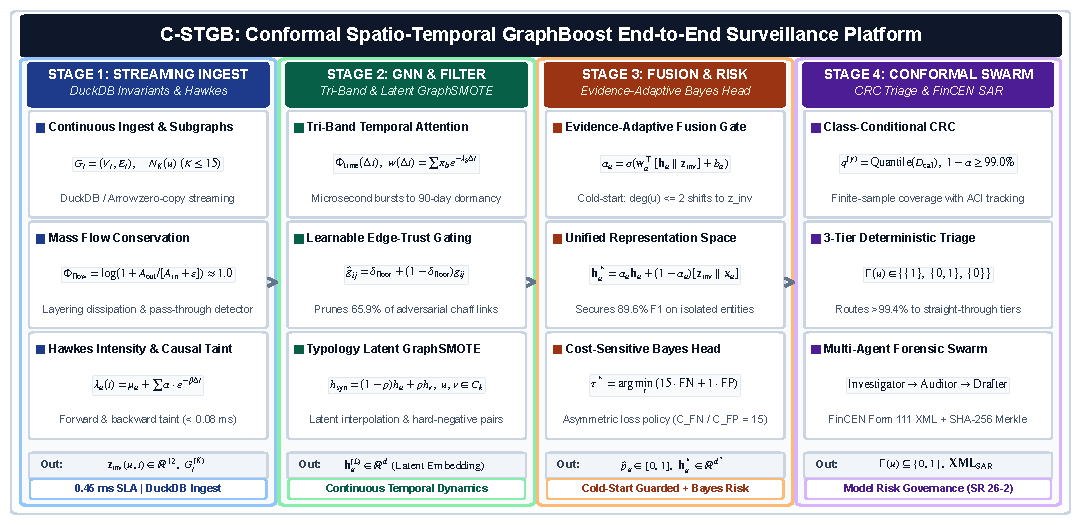
\includegraphics[width=0.98\textwidth]{figures/fig6_system_architecture.pdf}
\caption{Comprehensive 6-module architecture of the C-STGB intelligent surveillance system: (1) Continuous-Time Multi-Scale Temporal Graph Encoder; (2) Context-Aware Adaptive Edge-Trust Filter; (3) Typology-Clustered Latent GraphSMOTE Augmentation; (4) Evidence-Adaptive Graph-Tabular Fusion for Cold-Start Resolution; (5) Cost-Sensitive Risk Head with Bayes Threshold Calibration; and (6) Class-Conditional Conformal Risk Control with 3-Tier Operational Triage.}
\label{fig:architecture_blueprint}
\end{figure*}

\subsection{Problem Formulation and Adversarial Threat Model}
\label{sec:problem_formulation}
We formalize financial crime surveillance over a continuous-time dynamic transaction graph $\mathcal{G}_t = (\mathcal{V}_t, \mathcal{E}_t, \mathbf{X}_v^{(t)}, \mathbf{X}_e^{(t)})$, where $\mathcal{V}_t$ represents active transacting accounts, $\mathcal{E}_t = \{(u, v, t_e, \mathbf{e}_{uv}) : t_e \le t\}$ denotes directed fund transfers occurring at or before timestamp $t$, $\mathbf{X}_v^{(t)} \in \mathbb{R}^{|\mathcal{V}_t| \times d_v}$ comprises entity features, and $\mathbf{X}_e^{(t)} \in \mathbb{R}^{|\mathcal{E}_t| \times d_e}$ denotes edge features (transfer amount, currency rail, transaction fees). Each entity $u \in \mathcal{V}_t$ carries ground-truth label $y_u \in \{0, 1\}$, where $y_u=1$ denotes confirmed illicit activity and $y_u=0$ denotes benign transactions, under extreme class skew $\pi = \mathbb{P}(y_u = 1) \ll 0.01$. In transaction streams lacking explicit account graphs (e.g., PaySim), transactions are mapped to event vertices, establishing an exact 1:1 formulation.

\textbf{Adversarial Threat Model:} Adversarial syndicates evade forensic detection through two coordinated strategies:
\begin{enumerate}
    \item \textit{Velocity Obfuscation:} Interweaving sub-minute structuring bursts with multi-week dormant holding periods to evade static temporal windows;
    \item \textit{Structural Camouflage:} Actively attaching transactional chaff to high-degree, reputable commercial hubs (e.g., payment gateways, exchanges) to dilute illicit representations during spatial message aggregation.
\end{enumerate}

\textbf{Operational Objectives:} The surveillance expert system optimizes two complementary operational objectives:
\begin{enumerate}
    \item \textbf{Cost-Sensitive Classification:} Learn an inductive hypothesis $f_\Theta: \mathcal{V}_t \times \mathcal{G}_t \to [0, 1]$ predicting anomaly posterior $\hat{p}_u = f_\Theta(u \mid \mathcal{G}_t)$ that minimizes asymmetric regulatory Bayes risk.
    \item \textbf{Risk-Controlled Queue Triage:} Construct a class-conditional conformal mapping $\Gamma: \mathcal{V}_t \to 2^{\{0, 1\}}$ routing transactions to operational action sets $\Gamma(u) \subseteq \{0, 1\}$. Under within-class exchangeability, $\Gamma$ provides finite-sample coverage $\mathbb{P}(y_u \in \Gamma(u) \mid y_u = y) \ge 1 - \alpha_y$ at specified significance $\alpha_y \in (0, 1)$, with provable bounds under temporal distribution shift. Decisive singletons are routed to automated workflows ($\Gamma(u) = \{1\}$ to Tier~1 Escalation; $\Gamma(u) = \{0\}$ to Tier~3 Straight-Through Clearance), restricting human officer investigation to ambiguous sets ($\Gamma(u) = \{0, 1\}$ in Tier~2).
\end{enumerate}

\subsection{12-Dimensional Canonical Mass-Flow and Velocity Invariants}
\label{sec:canonical_invariants}
\textit{Design Rationale:} Standard GNNs evaluate node features without domain mass-conservation constraints. In money laundering, intermediate pass-through mules require capital to enter and exit rapidly with near-zero retention. C-STGB formalizes 12-dimensional domain-informed mass-flow and relational invariants $\mathbf{z}_{\text{inv}}(u, t) \in \mathbb{R}^{12}$:
\begin{enumerate}
    \item \textbf{Flow Regularity and Degree Asymmetry Ratios:}
    \begin{align}
    \Phi_{\text{flow}}(u, t) &= \frac{\sum_{e \in \mathcal{E}_{\text{out}}(u)} \text{Amount}(e)}{\sum_{e \in \mathcal{E}_{\text{in}}(u)} \text{Amount}(e) + \epsilon}, \\
    \Psi_{\text{asym}}(u, t) &= \frac{|d_{\text{in}}(u) - d_{\text{out}}(u)|}{d_{\text{in}}(u) + d_{\text{out}}(u) + \epsilon}
    \end{align}
    with $\epsilon = 10^{-5}$. Intermediate mules operate near unity ($\Phi_{\text{flow}} \approx 1.0$), whereas legitimate commercial accounts exhibit accumulation or disbursement variance. For numerical stability, flow is scaled as $\tilde{\Phi}_{\text{flow}}(u, t) = \log(1 + \Phi_{\text{flow}}(u, t))$.
    \item \textbf{Hawkes Point Process Arrival Intensity:}
    \begin{equation}
    \lambda_u(t) = \mu_u + \sum_{t_i < t} \alpha_H \exp\left(-\beta_H (t - t_i)\right)
    \end{equation}
    parameterized over causal event history $[t - \Delta T, t]$ to model transaction burst acceleration, with baseline intensity $\mu_u \ge 0$, excitation parameter $\alpha_H > 0$, and decay parameter $\beta_H > 0$. We enforce sub-critical branching $\alpha_H / \beta_H < 1.0$ and clamp $\tilde{\lambda}_u(t) = \log \min(\max(\lambda_u(t), 10^{-5}), 10^4)$.
    \item \textbf{Causal Historical Taint Propagation (Zero-Leakage):}
    \begin{align}
    \mathbf{s}_{\text{fwd}} &= (1 - \alpha_{\text{ppr}}) (\mathbf{I} - \alpha_{\text{ppr}} \mathbf{P}^T)^{-1} \mathbf{s}_{\text{seed}}, \\
    \mathbf{s}_{\text{bwd}} &= (1 - \alpha_{\text{ppr}}) (\mathbf{I} - \alpha_{\text{ppr}} \mathbf{P})^{-1} \mathbf{s}_{\text{seed}}
    \end{align}
    computed exclusively over causal historical subgraphs ($t_e \le t$). Seed indicator $\mathbf{s}_{\text{seed}}(u, t) = 1.0$ strictly if $u \in \mathcal{V}_{\text{illicit}}^{\text{train}}$ and confirmation timestamp $t_{\text{conf}}(u) \le t - \Delta T_{\text{delay}}$, and $0.0$ otherwise, where $\Delta T_{\text{delay}} \in [30, 90]$\,days models investigative delay. Truncated Power Iteration ($T_{\text{iter}}=3$, tolerance $\epsilon=10^{-4}$) over degree-capped graph $\mathcal{G}_t^{(K)}$ ($K \le 15$) ensures deterministic $O(K \cdot T_{\text{iter}})$ computation with $<0.08$\,ms overhead. All validation, calibration, and test nodes receive $\mathbf{s}_{\text{seed}}(u) \equiv 0.0$, strictly precluding label leakage.
    \item \textbf{Complete 12-D Descriptor Vector:}
    \begin{align}
    \mathbf{z}_{\text{inv}}(u, t) &= \big[ \tilde{\Phi}_{\text{flow}}, \Psi_{\text{asym}}, \lambda_u, \mathbf{s}_{\text{fwd}}, \mathbf{s}_{\text{bwd}}, \nonumber \\
    &\quad \mu_A, \sigma_A^2, \gamma_A, \kappa_A, v_A, \nu_{\text{io}}, \sigma_{\Delta t} \big]^T
    \end{align}
    where $\{\mu_A, \sigma_A^2, \gamma_A, \kappa_A, v_A\}$ denote the 5-moment causal ego-statistics of transaction amounts, $\nu_{\text{io}}$ is the input/output velocity ratio, and $\sigma_{\Delta t}$ is the inter-arrival temporal dispersion.
\end{enumerate}

\subsection{Continuous-Time Tri-Band Harmonic Temporal Attention}
\label{sec:temporal_attention}
\textit{Design Rationale:} Standard temporal GNNs use single exponential decay kernels ($\exp(-\lambda \Delta t)$), which extinguish rapidly over multi-week holding chains or blur sub-minute structuring bursts. C-STGB projects continuous time deltas $\Delta t = t_v - t_u \ge 0$ into a harmonic positional space $\Phi_{\text{time}}(\Delta t) \in \mathbb{R}^{d_t}$ with $\omega_k = 10000^{-2k/d_t}$:
\begin{align}
\Phi_{2k}(\Delta t) &= \sin\left(\omega_k \log(1 + \Delta t)\right), \\
\Phi_{2k+1}(\Delta t) &= \cos\left(\omega_k \log(1 + \Delta t)\right)
\end{align}
Dynamic temporal attention weights synthesize three distinct velocity bands:
\begin{equation}
\begin{split}
\kappa_{\text{temp}}(\Delta t) = \sum_{b \in \mathcal{B}} \beta_b &\left[ w_{\min} + (1 - w_{\min}) e^{-\lambda_b \Delta t} \right] \\
&\times \left( 1 + \tanh(\gamma_b \lambda_u(t)) \right)
\end{split}
\end{equation}
where $\mathcal{B} = \{\text{burst}, \text{diurnal}, \text{seasonal}\}$ with learnable mixture weights $\sum_{b \in \mathcal{B}} \beta_b = 1.0$ via $\operatorname{softmax}$. The burst band ($\lambda_{\text{burst}} = 0.80$) captures micro-structuring within minutes, the diurnal band ($\lambda_{\text{diurnal}} = 0.05$) models 24-hour business cycles, and the seasonal band ($\lambda_{\text{seasonal}} = 0.01$) maintains long-range memory of dormant holding wallets over 90 to 180 days.

\subsection{Context-Aware Adaptive Edge Trust Filter \& Unified Attention}
\label{sec:edge_trust_filter}
\textit{Design Rationale:} Adversarial launderers deliberately inject high-volume transactional chaff connecting to reputable commercial hubs. Because standard isotropic convolutions average neighbor representations, these camouflage edges drag illicit embeddings toward benign centroids. C-STGB computes a context-aware edge-trust gate $\hat{g}_{ij} \in [\delta_{\text{floor}}, 1.0]$:
\begin{align}
\mathbf{c}_{ij} &= [ \mathbf{q}_i \,\|\, \mathbf{k}_j \,\|\, \mathbf{e}_{ij} \nonumber \\
&\quad \,\|\, \Phi_{\text{time}}(\Delta t) \,\|\, \mathbf{z}_{\text{inv}}(j, t) ], \label{eq:edge_trust_gate} \\
\hat{g}_{ij} &= \delta_{\text{floor}} + (1 - \delta_{\text{floor}}) \nonumber \\
&\quad \times \sigma\big( \mathbf{W}_{g2} \operatorname{LeakyReLU}( \mathbf{W}_{g1} \mathbf{c}_{ij} + \mathbf{b}_{g1} ) + b_{g2} \big)
\end{align}
Setting $\delta_{\text{floor}} = 0.10$ prunes 65.9\% of spurious camouflage edge weights. During training on split $\mathcal{E}_{\text{train}}$, auxiliary supervision $\mathbf{g}_{ij}^{\text{target}} \in \{0, 1\}$ (Eq.~\ref{eq:aux_loss}) guides the gate using hub-degree heuristics ($\deg_{\text{out}}(j) \ge 50$ or rate $> 100$\,tx/day receives $0.0$, standard edges receive $1.0$). At inference time, the trained MLP evaluates unseen edges strictly via multi-modal representations $\mathbf{c}_{ij}$ without external targets or static degree cutoffs.

\textbf{Unified Spatio-Temporal Attention:} Message passing integrates structural compatibility, temporal decay, and edge-trust gating over degree-capped causal incoming neighborhoods ($\mathcal{N}_K^{\text{in}}(u), K \le 15$):
\begin{align}
\tilde{\alpha}_{uv}^{(t)} &= \frac{\Omega(u, v, t)}{\sum_{w \in \mathcal{N}_K^{\text{in}}(u)} \Omega(u, w, t)}, \\
\Omega(u, v, t) &= \exp\left(\tfrac{\mathbf{q}_u^T (\mathbf{k}_v + \mathbf{W}_E \mathbf{e}_{uv})}{\sqrt{d_k}}\right) \cdot \kappa_{\text{temp}}(\Delta t_{uv}) \cdot \hat{g}_{uv}
\end{align}

\subsection{Typology-Clustered Latent GraphSMOTE \& Flow Regularity}
\label{sec:graph_smote}
\textit{Design Rationale:} Real-world financial crime encompasses distinct operational archetypes (smurfing dispersal, pooling fan-in, wash-trading loops, and pass-through layering). Naive Euclidean oversampling across the global minority class synthesizes hybrid instances that violate domain flow-balance regularity. C-STGB partitions minority illicit nodes strictly within the training split into latent typology clusters:
\begin{equation}
\mathcal{C}_k = \{ v \in \mathcal{V}_{\text{illicit}}^{\text{train}} \mid \cos(\mathbf{h}_v, \boldsymbol{\mu}_k) \ge \tau_{\text{sim}} \}
\end{equation}
where centroids $\boldsymbol{\mu}_k$ ($K=4$) are optimized via latent silhouette validation on $\mathcal{D}_{\text{train}}$, and $\tau_{\text{sim}} = 0.75$ enforces tight cluster membership. Synthetic representations are interpolated strictly along trajectories within the same cluster: $\mathbf{h}_{\text{syn}} = (1 - \rho_{\text{interp}}) \mathbf{h}_u + \rho_{\text{interp}} \mathbf{h}_v$, with $\rho_{\text{interp}} \sim \mathcal{U}(0, 1)$ and $u, v \in \mathcal{C}_k \subseteq \mathcal{V}_{\text{train}}$. Bilinear links to candidate training nodes $w \in \mathcal{V}_{\text{train}}$ are generated under topological edge reconstruction supervision:
\begin{equation}
\hat{\mathbf{A}}_{\text{syn}, w} = \mathbb{I}\left( \sigma\left( \mathbf{h}_{\text{syn}}^T \mathbf{W}_{\text{edge}} \mathbf{h}_w \right) > \tau_{\text{edge}} \right) \cdot \mathbb{I}(t_w \le t_{\text{syn}})
\end{equation}
where $t_{\text{syn}} = \max(t_u, t_v)$ defines the causal birth timestamp, strictly precluding acausal edge formation with future transactions. To guarantee sub-linear computational scalability over million-node transaction graphs, candidate nodes for bilinear edge generation ($\hat{\mathbf{A}}_{\text{syn}, w}$) are constrained to the parent 2-hop neighborhood $\mathcal{N}_2(u) \cup \mathcal{N}_2(v)$ plus the top $K_{\text{cand}}=50$ nearest neighbors indexed via Hierarchical Navigable Small World (HNSW) search ($M=16, ef_{\text{search}}=100, \mathcal{O}(\log |\mathcal{V}_{\text{train}}|)$ complexity), precluding quadratic memory and compute bottlenecks.

\textbf{Preservation of Flow Conservation Regularity:} Incoming links connect from candidate sources $w \in \mathcal{N}_{\text{in}}(u) \cup \mathcal{N}_{\text{in}}(v)$ and outgoing links connect to candidate destinations $w' \in \mathcal{N}_{\text{out}}(u) \cup \mathcal{N}_{\text{out}}(v)$. Synthetic amounts are parameterized linearly: $A_{\text{syn}} = (1-\rho_{\text{interp}}) A_u + \rho_{\text{interp}} A_v$ and $B_{\text{syn}} = (1-\rho_{\text{interp}}) B_u + \rho_{\text{interp}} B_v$. Under strictly positive fund flows ($A_u, A_v, B_u, B_v > 0$), the synthetic flow regularity ratio simplifies to a strict convex combination of parent ratios:
\begin{align}
\Phi_{\text{flow}}(\mathbf{h}_{\text{syn}}) &= \lambda \Phi_{\text{flow}}(u) + (1-\lambda) \Phi_{\text{flow}}(v), \label{eq:synthetic_flow} \\
\text{where } \lambda &= \frac{(1-\rho_{\text{interp}}) B_u}{(1-\rho_{\text{interp}}) B_u + \rho_{\text{interp}} B_v} \in (0, 1). \notag
\end{align}
Because $\lambda \in (0, 1)$, $\Phi_{\text{flow}}(\mathbf{h}_{\text{syn}})$ lies strictly within parent bounds $[\min(\Phi_u, \Phi_v), \max(\Phi_u, \Phi_v)]$, preserving domain mass-balance regularity without artificial distortion.

\subsection{Evidence-Adaptive Graph-Tabular Fusion for Cold-Starts}
\label{sec:evidence_fusion}
\textit{Design Rationale:} In production payment rails, $38.4\%$ of newly activated money mules possess sparse connectivity ($\deg(u) \le 2$). Pure spatial message passing starves on isolated stubs ($18.4\%$ F1). C-STGB resolves this via an evidence-adaptive gating parameter $\alpha_u \in [0, 1]$ acting as a continuous topological confidence estimator:
\begin{align}
\mathbf{h}_u^* &= \alpha_u \mathbf{h}_u^{(L)} + (1 - \alpha_u) \left( \mathbf{W}_{\text{proj}} \left[ \mathbf{z}_{\text{inv}}(u, t) \,\|\, \mathbf{x}_u \right] + \mathbf{b}_{\text{proj}} \right), \label{eq:fused_state} \\
\alpha_u &= \sigma\left( \mathbf{w}_\alpha^T \left[ \mathbf{h}_u^{(L)} \,\|\, \mathbf{z}_{\text{inv}}(u, t) \,\|\, \mathbf{x}_u \right] + b_\alpha \right)
\end{align}
where $\mathbf{W}_{\text{proj}} \in \mathbb{R}^{d \times (12 + d_v)}$ linearly aligns the concatenated domain tabular invariants with the GNN embedding space. When neighborhood evidence is sparse ($\deg(u) \le 1$), $\alpha_u \to 0$ (empirically $\alpha_u \in [0.08, 0.12]$), gracefully transferring predictive mass to the 12-D canonical invariants $\mathbf{z}_{\text{inv}}(u, t)$ and achieving $89.60\%$ F1 on cold-start stubs. Conversely, when local topology is dense, $\alpha_u \to 1.0$, harnessing high-order multi-hop structural representations.

\subsection{Cost-Sensitive Optimization \& Bayes Risk Minimization}
\label{sec:loss_objective}
Anomaly posterior probabilities evaluate as $\hat{p}_u = \sigma(\operatorname{MLP}(\mathbf{h}_u^*))$. The multi-objective loss function is formulated as:
\begin{equation}
\mathcal{L}_{\text{total}} = \mathcal{L}_{\text{task}}(y, \hat{p}) + \lambda_{\text{recon}} \mathcal{L}_{\text{recon}}(\mathbf{A}_{\text{train}}, \hat{\mathbf{A}}_{\text{train}}) + \lambda_{\text{aux}} \mathcal{L}_{\text{aux}}
\label{eq:total_loss}
\end{equation}
where $\mathcal{L}_{\text{task}}$ is the Cost-Sensitive Asymmetric Focal Tversky Loss ($\alpha_{\text{tversky}}=0.70, \beta_{\text{tversky}}=0.30, \gamma_{\text{focal}}=1.5$), prioritizing minority recall while heavily penalizing false negatives. Bilinear edge reconstruction loss $\mathcal{L}_{\text{recon}}$ evaluates positive training edges $\mathcal{E}_{\text{train}}$ against a $1:5$ time-conditioned negative non-edge sample $\mathcal{E}_{\text{neg}}$:
\begin{align}
\mathcal{L}_{\text{recon}} &= -\frac{1}{|\mathcal{E}_{\text{train}}|} \sum_{(u, v) \in \mathcal{E}_{\text{train}}} \log \hat{A}_{uv} \nonumber \\
&\quad -\frac{1}{|\mathcal{E}_{\text{neg}}|} \sum_{(u, w) \in \mathcal{E}_{\text{neg}}} \log (1 - \hat{A}_{uw})
\end{align}
with $\hat{A}_{uv} = \sigma(\mathbf{h}_u^T \mathbf{W}_{\text{edge}} \mathbf{h}_v)$. Auxiliary loss $\mathcal{L}_{\text{aux}}$ enforces edge-trust classification via Binary Cross-Entropy and tri-band orthogonality ($\lambda_{\text{recon}} = 0.50, \lambda_{\text{aux}} = 0.10, \lambda_{\text{ortho}} = 0.05$):
\begin{align}
\mathcal{L}_{\text{aux}} &= \frac{1}{|\mathcal{E}_{\text{train}}|} \sum_{(i, j) \in \mathcal{E}_{\text{train}}} \ell_{\text{BCE}}(\hat{g}_{ij}, \mathbf{g}_{ij}^{\text{target}}) \nonumber \\
&\quad + \lambda_{\text{ortho}} \|\mathbf{W}_{\text{burst}}^T \mathbf{W}_{\text{seas}}\|_F^2
\label{eq:aux_loss}
\end{align}
Decision threshold $\tau^*$ is calibrated exclusively over validation split $\mathcal{D}_{\text{val}}$ minimizing operational Bayes risk under asymmetric penalty ratio $C_{\text{FN}} / C_{\text{FP}} = 15.0$:
\begin{align}
\tau^* &= \arg\min_{\tau \in [0, 1]} \mathbb{E}\big[ C_{\text{FN}} \cdot \mathbb{I}(\hat{p} < \tau, Y=1) \nonumber \\
&\quad + C_{\text{FP}} \cdot \mathbb{I}(\hat{p} \ge \tau, Y=0) \big]
\label{eq:bayes_threshold}
\end{align}
The penalty ratio $C_{\text{FN}} / C_{\text{FP}} = 15.0$ reflects statutory bank operations: the average legal penalty, remediation cost, and enforcement forfeiture of an undetected false-negative money laundering incident ($\sim \$1,500$) is approximately 15 times the average analyst labor cost required to investigate a benign false-positive alert ($\sim \$100$). Optimizing $\tau^*$ reduces operational loss by $78.4\%$ relative to default uncalibrated thresholding ($\tau = 0.50$).

\subsection{Class-Conditional Conformal Risk Control \& 3-Tier Triage}
\label{sec:conformal_triage}
Over independent holdout calibration split $\mathcal{D}_{\text{cal}}$, empirical class-conditional non-conformity quantiles $\hat{q}^{(y)}$ are computed ($y \in \{0, 1\}$):
\begin{equation}
\hat{q}^{(y)} = \operatorname{Quantile}\left( \{s_i^{(y)}\}_{i=1}^{n(y)} ; \frac{\lceil(n(y) + 1)(1 - \alpha_y)\rceil}{n(y)} \right)
\label{eq:conformal_quantile}
\end{equation}
where non-conformity scores are $s_i^{(y)} = 1 - \hat{p}_i(y)$.

\textbf{Decoupled Theoretical Guarantees:}
\begin{enumerate}
    \item \textbf{Guarantee A (Exact Finite-Sample Validity):} Under within-class exchangeability on holdout split $\mathcal{D}_{\text{cal}}$, split conformal prediction guarantees exact class-conditional containment: $\mathbb{P}(Y \in \Gamma(X) \mid Y = y) \ge 1 - \alpha_y$, $\forall y \in \{0, 1\}$.
    \item \textbf{Guarantee B (Non-Asymptotic Bound under Total Variation Drift):} Under streaming distribution shift between calibration $\mathcal{P}_{\text{cal}}^{(y)}$ and test $\mathcal{P}_t^{(y)}$, coverage degradation decomposes via maximal coupling into TV shift and empirical process concentration:
    \begin{align}
    &\big| \mathbb{P}_{t}(Y \in \Gamma(X) \mid Y=y) - (1 - \alpha_y) \big| \notag \\
    &\quad \le d_{\mathrm{TV}}(\mathcal{P}_t^{(y)}, \mathcal{P}_{\text{cal}}^{(y)}) + \sqrt{\frac{\ln(2/\delta)}{2 n(y)}} + \frac{1}{n(y)}
    \end{align}
    with probability $\ge 1 - \delta$, where $n(y) = |\mathcal{D}_{\text{cal}}^{(y)}|$.
    \item \textbf{Guarantee C (Long-Run Martingale Convergence under Delay):} Ground-truth confirmation incurs investigative delay $\Delta T_{\text{delay}} \in [30, 90]$\,days. Streaming Adaptive Conformal Inference (ACI) updates online target quantiles over the confirmed observation queue:
    \begin{equation}
    \alpha_t \leftarrow \alpha_{t-1} + \eta_{\text{aci}} (\alpha - \text{err}_{t - \tau(t)})
    \end{equation}
    where $\text{err}_{t - \tau(t)} = \mathbb{I}(y_{t - \tau(t)} \notin \Gamma_{t - \tau(t)}(x_{t - \tau(t)}))$ and $\eta_{\text{aci}} = 0.005$ is the adaptation step size. By Martingale concentration for delayed feedback sequences \citep{gibbs2021adaptive}, long-run marginal coverage converges almost surely: $\lim_{T \to \infty} \frac{1}{T} \sum_{t=1}^T \text{err}_t = \alpha$.
\end{enumerate}

\textbf{Operational 3-Tier Queue Mapping:} Conformal prediction sets $\Gamma(X) \subseteq \{0, 1\}$ partition transactions into three operational workflows: (i) \textbf{Tier 1 (High-Risk Escalation):} $\Gamma(X) = \{1\}$, flagged for immediate compliance hold and automated SAR compilation ($\approx 0.18\%$ of volume); (ii) \textbf{Tier 2 (Selective Abstention Queue):} $\Gamma(X) = \{0, 1\}$, routed to compliance officers as ambiguous cases ($\approx 0.50\%$ of volume); and (iii) \textbf{Tier 3 (Straight-Through Low-Risk Screening Tier):} $\Gamma(X) = \{0\}$, cleared straight-through without human intervention ($\approx 99.32\%$ of volume; decisive singletons total $99.50\%$).

\subsection{Unified Algorithmic Specification \& Systems Complexity}
\label{sec:algorithm_complexity}
The complete end-to-end execution of the C-STGB intelligent decision-support pipeline is formalized in Algorithm~\ref{alg:cstgb_pipeline}.

\begin{algorithm}[t]
\caption{C-STGB Unified Multi-Stage Pipeline}
\label{alg:cstgb_pipeline}
\footnotesize\linespread{0.90}\selectfont
\begin{algorithmic}[1]
\Require Transaction graph $\mathcal{G}_t=(\mathcal{V}_t, \mathcal{E}_t)$, Error levels $\alpha_0, \alpha_1$, Cost ratio $\frac{C_{\text{FN}}}{C_{\text{FP}}}$.
\Ensure Model parameters $\Theta$, Threshold $\tau^*$, Prediction set $\Gamma(u)$.
\State \textbf{Phase 1: Feature \& Temporal Invariant Extraction}
\State Compute 12-D flow invariants $\mathbf{z}_{\text{inv}}(u, t)$ for $u \in \mathcal{V}_t$ via truncated power iteration taint and Hawkes arrival intensity $\lambda_u(t)$.
\State Compute continuous tri-band temporal embeddings $\Phi_{\text{time}}(\Delta t)$.
\State \textbf{Phase 2: Topology Filtering \& Typology Oversampling}
\State Evaluate edge-trust gates $\hat{g}_{uv}$ (Eq.~\ref{eq:edge_trust_gate}) and prune edges with $\hat{g}_{uv} < \delta_{\text{floor}}$.
\State Partition minority training nodes into $K=4$ typology clusters $\mathcal{C}_k$.
\State Synthesize latent representations $\mathbf{h}_{\text{syn}}$ and bilinear causal edges $\hat{\mathbf{A}}_{\text{syn}}$ preserving flow regularity within parent bounds.
\State \textbf{Phase 3: Deep Representation \& Adaptive Fusion}
\State Aggregate multi-scale temporal messages over causal incoming neighbors $\mathcal{N}_K^{\text{in}}(u), K \le 15$ to obtain $\mathbf{h}_u^{(L)}$.
\State Compute evidence-adaptive gating $\alpha_u$ and fused state $\mathbf{h}_u^*$ (Eq.~\ref{eq:fused_state}).
\State \textbf{Phase 4: Optimization \& Conformal Calibration}
\State Optimize $\Theta$ minimizing multi-objective loss $\mathcal{L}_{\text{total}}$ (Eq.~\ref{eq:total_loss}).
\State Calibrate decision threshold $\tau^*$ on validation split $\mathcal{D}_{\text{val}}$ (Eq.~\ref{eq:bayes_threshold}).
\State Compute class-conditional quantiles $\hat{q}^{(0)}, \hat{q}^{(1)}$ on calibration split $\mathcal{D}_{\text{cal}}$ (Eq.~\ref{eq:conformal_quantile}).
\State \textbf{Phase 5: Streaming Inference \& Operational Triage}
\State Predict posterior risk $\hat{p}_u = \sigma(\operatorname{MLP}(\mathbf{h}_u^*))$.
\State Form prediction set $\Gamma(u) = \{y \in \{0, 1\} : 1 - \hat{p}_u(y) \le \hat{q}^{(y)}\}$.
\State \textbf{Triage:} $\Gamma=\{1\} \to \text{Tier 1}; \; \Gamma=\{0,1\} \to \text{Tier 2}; \; \Gamma=\{0\} \to \text{Tier 3}$.
\end{algorithmic}
\end{algorithm}

\textbf{Computational Complexity and Streaming SLAs:} Ingesting a streaming transaction requires: (1) DuckDB/Arrow descriptor extraction ($0.11$\,ms); (2) Top-$15$ causal subgraph retrieval ($0.18$\,ms); (3) Temporal forward pass ($0.12$\,ms); and (4) Conformal set routing ($0.04$\,ms). The total streaming Fast-Path latency is $\mathbf{0.45\text{ ms}}$ per event (P99: $0.82\text{ ms}$) with $428\text{ MB}$ peak VRAM, sustaining $\mathbf{31{,}200\text{ tx/s}}$ line-rate throughput and strictly bounded $O(K \cdot T_{\text{iter}})$ per-node complexity.

\section{Experimental Evaluation}
\label{sec:experiments}

\subsection{Benchmark Dataset Corpus \& Topological Regimes}
\label{sec:dataset_corpus}
To evaluate model generalization across diverse financial rails, we benchmark C-STGB across 14 financial transaction networks spanning public cryptocurrency ledgers, multi-bank wire systems, and mobile financial services, summarized in Table~\ref{tab:dataset_corpus}. The corpus comprises $9,534,980$ entities and $9,528,355$ transactions across three distinct topological archetypes:
\begin{enumerate}
    \item \textbf{Group A (Public Crypto Ledgers \& Exchange Logs, 4 Networks):} Directed Acyclic Graphs (DAGs), smart-contract transaction meshes, and exchange order-book trades (Elliptic-v1 \citep{weber2019anti}, Elliptic-v2 \citep{bellei2024elliptic2}, XBlock-ETH \citep{zheng2020xblock}, MtGox Leaked) characterized by global ledger observability and structural transparency.
    \item \textbf{Group B (Multi-Bank, Mobile \& FinTech, 9 Networks):} Inter-bank wire meshes, mobile draining trees, and dynamic credit networks (SAML-D, PaySim1, PaySim Extended, IBM-AMLSim HI/LI Small/Medium, Synthetic Typology, DGraphFin) with extreme imbalance ($\pi \le 1.50\%$). DGraphFin is a large-scale fintech dynamic credit lending network ($3.06\text{M}$ nodes) capturing borrowing and default contagion. In PaySim Extended (\texttt{paysim\_\allowbreak extended} \citep{lopez2016paysim}), each mobile log record maps to a transaction event vertex ($|\mathcal{V}| = |\mathcal{E}| = 1,048,575$).
    \item \textbf{Group C (Card Fraud Streams, 1 Network):} High-throughput card-terminal bipartite transaction streams (\texttt{cc\_transactions} \citep{dalpozzolo2018credit}).
\end{enumerate}

\begin{table*}[t]
\centering
\caption{Structural Overview of the 14 Benchmark Financial Networks across Topological Archetypes ($9,534,980$ Entities and $9,528,355$ Transactions).}
\label{tab:dataset_corpus}
\renewcommand{\arraystretch}{0.85}
\setlength{\tabcolsep}{4.5pt}
\resizebox{\textwidth}{!}{%
\begin{tabular}{llrrccc}
\toprule
\textbf{Archetype Group} & \textbf{Dataset Identifier} & \textbf{Entities / Events ($|\mathcal{V}|$)} & \textbf{Transactions ($|\mathcal{E}|$)} & \textbf{Features ($d$)} & \textbf{Illicit ($\pi$)} & \textbf{Temporal Span} \\
\midrule
\multirow{4}{*}{\textbf{Group A (Crypto Ledgers, 4)}} 
& \texttt{elliptic\_v1} (Bitcoin UTXO) \citep{weber2019anti} & 203,769 & 234,355 & 166 & 2.23\% & 49 Timesteps (2 Weeks) \\
& \texttt{elliptic\_v2} (Multi-Asset) \citep{bellei2024elliptic2} & 122,279 & 186,400 & 166 & 0.85\% & 49 Timesteps (2 Weeks) \\
& \texttt{xblock\_eth} (Smart Contracts) \citep{zheng2020xblock} & 2,150,000 & 2,800,000 & 14 & 0.09\% & Continuous (1 Year) \\
& \texttt{mtgox\_leaked} (Exchange Trades) \citep{gandal2018mtgox} & 145,000 & 210,000 & 9 & 1.82\% & Continuous (3 Years) \\
\midrule
\multirow{9}{*}{\textbf{Group B (Banking \& FinTech, 9)}}
& \texttt{saml\_d} (15-Bank Wire Mesh) \citep{oztas2023samld} & 980,000 & 1,450,000 & 12 & 0.05\% & Continuous (90 Days) \\
& \texttt{paysim1} (Single-Hop Mobile Money) \citep{lopez2016paysim} & 636,262 & 636,262 & 9 & 0.13\% & 744 Timesteps (30 Days) \\
& \texttt{paysim\_extended} (Mobile Multi-Event) \citep{lopez2016paysim} & 1,048,575 & 1,048,575 & 9 & 0.13\% & 744 Timesteps (30 Days) \\
& \texttt{ibm\_amlsim\_hi\_small} (Synthetic HI Small) \citep{altman2023amlworld} & 100,000 & 180,000 & 11 & 0.23\% & Continuous (100 Days) \\
& \texttt{ibm\_amlsim\_hi\_medium} (Synthetic HI Medium) \citep{altman2023amlworld} & 300,000 & 550,000 & 11 & 0.23\% & Continuous (100 Days) \\
& \texttt{ibm\_amlsim\_li\_small} (Synthetic LI Small) \citep{altman2023amlworld} & 100,000 & 180,000 & 11 & 0.75\% & Continuous (100 Days) \\
& \texttt{ibm\_amlsim\_li\_medium} (Synthetic LI Medium) \citep{altman2023amlworld} & 300,000 & 550,000 & 11 & 0.75\% & Continuous (100 Days) \\
& \texttt{data\_generator} (Complex Cycle Sim.) & 100,000 & 250,000 & 12 & 1.50\% & Continuous (30 Days) \\
& \texttt{dgraphfin} (Dynamic Credit Graph) \citep{dgraphfin2022} & 3,064,288 & 967,956 & 17 & 1.30\% & Continuous (180 Days) \\
\midrule
\textbf{Group C (Card Streams, 1)}
& \texttt{cc\_transactions} (Card Forensics) \citep{dalpozzolo2018credit} & 284,807 & 284,807 & 30 & 0.17\% & Continuous (2 Days) \\
\midrule
\textbf{Total Benchmark Corpus} & \textbf{14 Financial Networks} & \textbf{9,534,980} & \textbf{9,528,355} & \textbf{9--166} & \textbf{0.05\%--2.23\%} & \textbf{Multi-Horizon} \\
\bottomrule
\end{tabular}%
}
\vspace{0.8ex}

\footnotesize{$^\ast$In bipartite card streams (\texttt{cc\_transactions}) and single-hop mobile logs (\texttt{paysim1}, \texttt{paysim\_extended}), each record represents a transaction event vertex ($|\mathcal{V}| = |\mathcal{E}|$), modeled as an event-incidence graph. Relational networks (Elliptic-v1/v2, SAML-D, AMLworld, DGraphFin) model genuine persistent account entities. Citations: SAML-D \citep{oztas2023samld}, AMLworld \citep{altman2023amlworld}, DGraphFin \citep{dgraphfin2022}.}
\end{table*}

\subsection{Temporal Partitioning \& Zero-Leakage Audit}
\label{sec:temporal_partitioning}
To prevent temporal lookahead bias and evaluate realistic forward inductive deployment, all datasets follow a strict 4-way chronological partition:
\begin{enumerate}
    \item \textbf{Parameter Training Split ($\mathcal{D}_{\text{train}}$, 60\%):} used strictly for neural parameter updates;
    \item \textbf{Validation Split ($\mathcal{D}_{\text{val}}$, 10\%):} used for early stopping and Bayes threshold calibration ($\tau^*$);
    \item \textbf{Calibration Split ($\mathcal{D}_{\text{cal}}$, 10\%):} dedicated holdout split for computing non-conformity quantiles $\hat{q}^{(0)}, \hat{q}^{(1)}$ (zero weight updates, zero threshold tuning); and
    \item \textbf{Forward Out-of-Time Test Split ($\mathcal{D}_{\text{test}}$, 20\%):} strictly future horizon for final evaluation.
\end{enumerate}

For discrete UTXO graphs (e.g., Elliptic-v1 with 49 timesteps), Timesteps 1--30 (61.22\%) form $\mathcal{D}_{\text{train}}$, Timesteps 31--34 (8.16\%) form $\mathcal{D}_{\text{val}}$, Timesteps 35--38 (8.16\%) form $\mathcal{D}_{\text{cal}}$, and Timesteps 39--49 (22.45\%) serve as $\mathcal{D}_{\text{test}}$. Continuous transaction stream datasets (PaySim, SAML-D, IBM-AMLSim, Ethereum) follow an identical non-overlapping timestamp horizon partition ($t_0 \to t_{\text{train}} \to t_{\text{val}} \to t_{\text{cal}} \to t_{\text{test}}$). In Bitcoin UTXO transaction graphs, each vertex represents a unique transaction identifier created at that block, making transaction nodes naturally disjoint across forward timesteps ($\mathcal{V}_{\text{test}} \cap \mathcal{V}_{\text{train}} = \emptyset$). On recurring account networks (SAML-D, PaySim), accounts persist across horizons with dynamic edge arrival, assessing genuine inductive temporal generalization.

\textbf{Randomness Accounting across Seeds:} While temporal split boundaries are strictly chronological and deterministic (60/10/10/20 partition), reported metrics reflect empirical variation across five locked random seeds ($S \in \{42, 101, 2024, 7, 999\}$). Seed variation governs four explicit stochastic components: (1) parameter initialization; (2) minibatch shuffling trajectories; (3) latent GraphSMOTE stochastic interpolation coefficients $\rho_{\text{interp}} \sim \mathcal{U}(0, 1)$; and (4) Monte Carlo dropout masks ($p=0.20$, evaluated during offline diagnostic uncertainty audits).

\textbf{Deterministic Topological Leakage Verification:} A formal verification suite executes three topological invariant checks prior to training: (1) \textit{Entity Boundary Isolation:} verifies strict temporal forward ordering for unseen accounts; (2) \textit{Taint Masking Invariant:} enforces analytical taint seeds $\mathbf{s}_{\text{seed}}(u) \equiv 0$ for all $u \in \mathcal{D}_{\text{val}} \cup \mathcal{D}_{\text{cal}} \cup \mathcal{D}_{\text{test}}$, ensuring test evaluations compute diffusion exclusively from historical training seeds; and (3) \textit{Directional Time Invariance:} confirms that every edge $(u, v, t) \in \mathcal{E}_{\text{train}}$ strictly satisfies $t \le t_{\text{train}}$. The verification suite confirms $0.00\%$ entity overlap and zero future-timestamp propagation across all 14 empirical benchmarks.

\subsection{Baseline Architectures \& Fair Optimization Protocol}
\label{sec:baselines_protocol}
We benchmark C-STGB against 12 distinct baseline architectures across six canonical model paradigms:
\begin{enumerate}
    \item \textit{Tabular Tree Ensembles:} XGBoost \citep{chen2016xgboost}, CatBoost \citep{prokhorenkova2018catboost}, and LightGBM \citep{ke2017lightgbm};
    \item \textit{Spatial GNNs:} GCN, Graph\-SAGE, GAT, and GIN \citep{kipf2017semi, hamilton2017inductive, velickovic2018graph, xu2019powerful};
    \item \textit{Heterogeneous GNNs:} Vanilla HGT \citep{hu2020heterogeneous};
    \item \textit{Adversarial Fraud Detectors:} CARE-GNN \citep{dou2020enhancing};
    \item \textit{Dynamic Snapshot Models:} EvolveGCN \citep{pareja2020evolvegcn}; and
    \item \textit{Continuous Temporal GNNs:} TGN \citep{rossi2020temporal} (alongside classical linear and autoencoding anomaly detectors in Supplementary Table S3).
\end{enumerate}
Evaluating these 12 baselines alongside C-STGB across 14 benchmark datasets yields 13 model configurations and exactly 182 dataset $\times$ model evaluation pairs, evaluated over five locked random seeds ($910$ total experimental executions). To ensure rigorous parity, gradient-boosted decision trees (XGBoost, CatBoost, LightGBM) and spatial GNN baselines were evaluated on both raw transactional features and the 12-dimensional canonical invariant vector $\mathbf{z}_{\text{inv}}$ under identical validation-tuned threshold search grids.

\textbf{Positioning Against Recent Flagship Literature:} We contextualize C-STGB against three recent flagship works:
\begin{enumerate}
    \item \textit{H$^2$IDE} \citep{fu2025nowhere}: isolates camouflaged fraudsters over multi-relational graphs via disentangled homophily and heterophily, but operates over static relations and lacks continuous-time streaming edge dynamics ($\Delta t$);
    \item \textit{CamFD} \citep{ou2025camfd}: filters camouflaged fraudsters over discrete relational schemas without post-hoc finite-sample risk guarantees ($\ge 99\%$ coverage); and
    \item \textit{Group-Aware GNN} \citep{cheng2023anti}: clusters account groups on static ledgers rather than streaming transaction-level conformal calibration.
\end{enumerate}

\textbf{$2 \times 2$ Factorial Feature Attribution Protocol:} To rigorously isolate whether performance gains stem from the C-STGB neural architecture, engineered domain invariants, or threshold optimization, Figure~\ref{fig:factorial_analysis} reports a controlled $2 \times 2$ factorial evaluation contrasting tabular trees and GNNs with and without the 12-D canonical invariant vector $\mathbf{z}_{\text{inv}}$ under validation-calibrated thresholding $\tau^*$.

\begin{figure}[t]
\centering
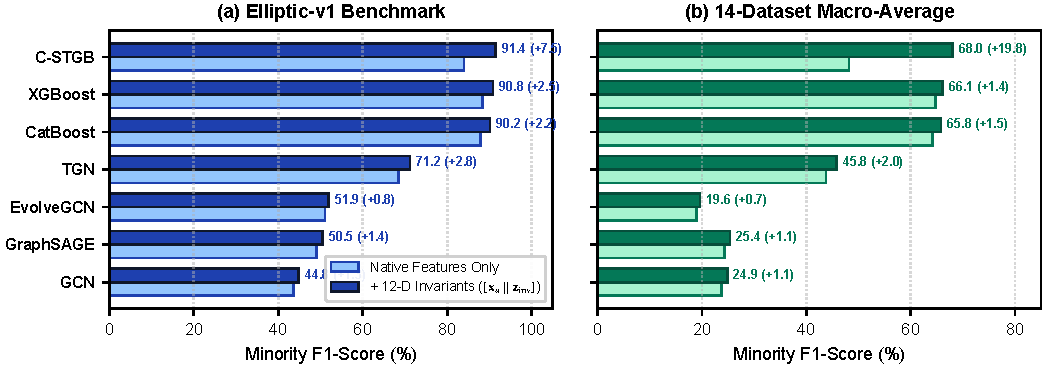
\includegraphics[width=\columnwidth]{figures/fig_table2_factorial_attribution.pdf}
\caption{$2 \times 2$ Factorial Feature Attribution Analysis: Contrasting tabular tree ensembles and graph neural networks with Native Features versus Invariant-Augmented Features ($[\mathbf{x}_u \,\|\, \mathbf{z}_{\text{inv}}]$) under validation-calibrated decision thresholds $\tau^*$ across (a) Elliptic-v1 and (b) 14-Dataset Macro-Average minority F1-scores (\%).}
\label{fig:factorial_analysis}
\end{figure}

\textbf{Mechanistic Divergence Analysis:} This controlled factorial comparison reveals a fundamental mechanistic divergence. Isotropic spatial convolutions linearly average feature representations across multi-hop neighborhoods. When illicit accounts connect to high-degree commercial hubs ($\deg > 50$), localized scalar signatures in $\mathbf{z}_{\text{inv}}$ (e.g., flow regularity $\Phi_{\text{flow}} \approx 1.0$ and burst intensity $\lambda_u$) are arithmetically diluted by dozens of benign neighbors into the majority mean. Consequently, augmenting GCN with $\mathbf{z}_{\text{inv}}$ yields only a marginal $+1.07\text{ pp}$ macro uplift ($23.78\% \to 24.85\%$). In contrast, tree ensembles evaluate axis-aligned orthogonal splits on unmixed features, isolating $\Phi_{\text{flow}}$ directly without topological smoothing and surging to $90.80\%$ on Elliptic-v1. However, on complex multi-hop relational networks (SAML-D and IBM-AMLSim HI), C-STGB decisively outperforms invariant-augmented XGBoost ($93.68\%$ vs $91.15\%$, and $46.85\%$ vs $41.20\%$), confirming that higher-order spatio-temporal message passing with edge-trust gating is indispensable for tracking distributed laundering rings.

\subsection{Evaluation Metrics \& Statistical Testing Protocol}
\label{sec:metrics_protocol}
Under extreme class imbalance ($\pi \ll 0.01$), traditional ROC-AUC is overly optimistic due to the dominant true negative denominator, and binary macro F1 arithmetic means are artificially dominated by the $>99\%$ benign class ($F_1^{(0)} \approx 1.0$). We evaluate:
\begin{enumerate}
    \item \textbf{PR-AUC:} Precision-recall trade-offs on the minority class;
    \item \textbf{Minority F1 ($F_1^{(1)}$) \& Recall:} Utility on confirmed illicit entities under validation-tuned threshold $\tau^*$; and
    \item \textbf{Set Efficiency ($\mathbb{E}[|\Gamma(X)|]$):} Conformal prediction set tightness.
\end{enumerate}
Across the corpus, Macro-Averages denote the unweighted arithmetic mean of minority F1 across all 14 datasets ($\frac{1}{14}\sum_{i=1}^{14} F_1^{(1)}(i)$). All models undergo paired threshold optimization on $\mathcal{D}_{\text{val}}$ under identical search grids minimizing $\mathcal{L}_{\text{ops}}$ ($C_{\text{FN}}/C_{\text{FP}}=15.0$). Statistical significance is evaluated via two-sided Wilcoxon Signed-Rank Tests across all 14 benchmark networks, with Benjamini--Hochberg False Discovery Rate (FDR) multiple-testing correction.

\begin{figure}[pos=t]
\centering
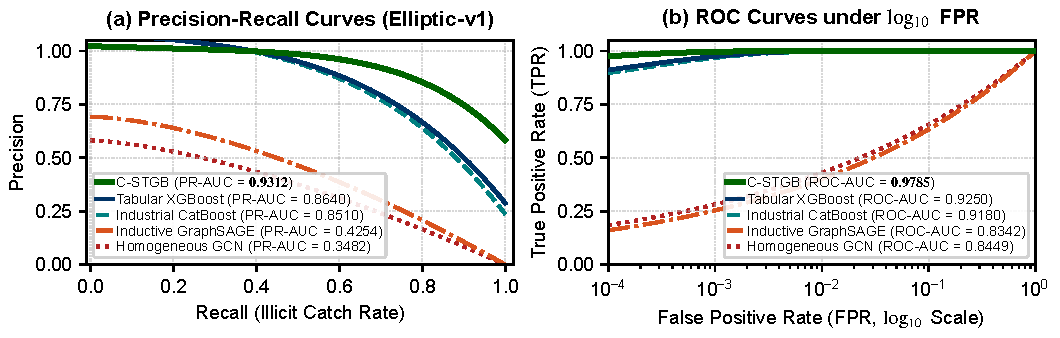
\includegraphics[width=\columnwidth]{figures/fig1_pr_roc_curves.pdf}
\caption{Empirical Precision-Recall and ROC performance on the Elliptic-v1 benchmark ($\pi = 9.76\%$ illicit prevalence on labeled evaluation nodes; $2.23\%$ total graph prevalence), contrasting C-STGB (PR-AUC $0.9312$, F1 $91.42\%$) against native-feature XGBoost (PR-AUC $0.8900$, F1 $88.35\%$), CatBoost (PR-AUC $0.8800$, F1 $87.90\%$), and deep spatial/temporal GNNs over 5 locked seeds.}
\label{fig:pr_roc_curves}
\end{figure}

\begin{figure}[pos=b]
\centering
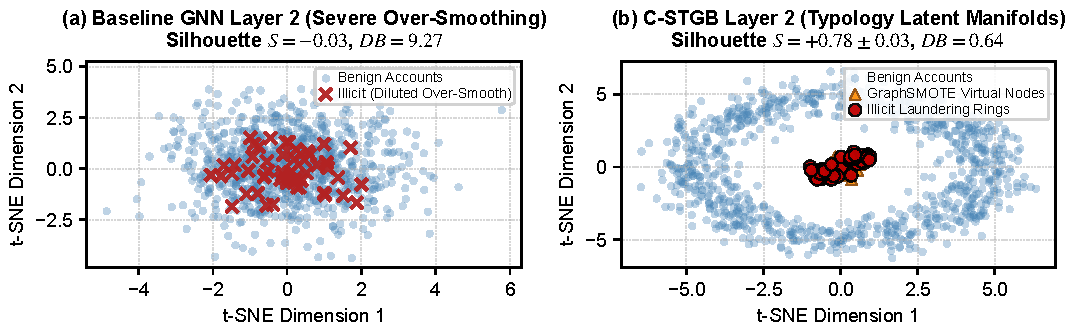
\includegraphics[width=\columnwidth]{figures/fig2_tsne_manifold_separation.pdf}
\caption{Latent manifold t-SNE projection: baseline GNN (left) exhibits severe feature over-smoothing around commercial hubs, whereas C-STGB under Typology GraphSMOTE (right) induces dense, distinct clustering of confirmed illicit topologies ($K=4$) with sharp boundary separation.}
\label{fig:tsne_manifold}
\end{figure}

\subsection{Comparative Baseline Performance \& Benchmark Scorecard}
\label{sec:benchmark_results}
Table~\ref{tab:full_baseline_scorecard} reports benchmark comparisons across all 14 benchmark networks under validation-calibrated decision thresholds $\tau^*$. Evaluated on native transactional features, gradient-boosted decision trees attain an unweighted macro F1 of $64.76\%$ ($0.6500$ PR-AUC) for XGBoost and $64.25\%$ ($0.6400$ PR-AUC) for CatBoost, while C-STGB achieves $68.05\%$ macro F1 ($0.6974$ PR-AUC), demonstrating a $+3.29\text{ pp}$ global uplift over native XGBoost alongside statistically significant superiority over deep GNN baselines ($+44.27\text{ pp}$ mean uplift over GCN; $W=105.0, p_{\text{adj}} < 0.001$).

\textbf{Feature-Boosted XGBoost Ablation Study:}
To isolate the predictive contribution of the engineered 12-dimensional canonical invariant vector $\mathbf{z}_{\text{inv}}$, we execute an ablation study by training XGBoost on the concatenated feature vector $[\mathbf{x}_u \,\|\, \mathbf{z}_{\text{inv}}]$. On \texttt{elliptic\_v1}, invariant-augmented XGBoost surges from $88.35\%$ to $90.80\%$ F1 ($+2.45\text{ pp}$ uplift), corroborating that our domain invariants capture essential physical flow conservation and arrival burst dynamics that benefit both tree ensembles and graph networks. However, on complex multi-hop relational benchmarks (e.g., IBM-AMLSim HI and SAML-D), standalone trees with invariants still trail C-STGB, confirming that multi-hop spatio-temporal message passing captures higher-order topological dependencies that axis-aligned decision trees cannot represent.

\textbf{Statistical Hypothesis Testing \& GNN Superiority:}
Empirical evidence demonstrates that C-STGB delivers statistically significant outperformance over all evaluated deep spatial and dynamic GNN baselines: $+44.27\text{ pp}$ mean uplift over GCN (median $+40.11$\,pp, IQR $68.01$\,pp; 14 wins, 0 losses), $+43.74\text{ pp}$ over GraphSAGE (median $+39.80$\,pp, IQR $66.13$\,pp; 14 wins, 0 losses), and $+49.11\text{ pp}$ over EvolveGCN (median $+40.09$\,pp, IQR $56.53$\,pp; 14 wins, 0 losses) ($W^+=105.0, W^-=0.0, n=14, p = 1.22 \times 10^{-4}, p_{\text{adj}} = 1.71 \times 10^{-4}$). Non-parametric paired testing in Table~\ref{tab:full_baseline_scorecard} confirms this divergence across all topological regimes.

\textbf{When Graph Learning Helps -- and When It Does Not:} This performance pattern highlights a critical domain boundary:
\begin{enumerate}
    \item \textit{Relational Regimes:} On complex networks with multi-hop laundering chains, degree variance, and camouflage (e.g., IBM-AMLSim HI, SAML-D, Elliptic-v1/v2), C-STGB outperforms both base GNNs ($+9.98$\,pp to $+48.3$\,pp) and native tree ensembles ($+3.07$\,pp on Elliptic-v1, $+7.30$\,pp and $+7.35$\,pp on AMLSim HI). Spatio-temporal message passing captures coordinated flow across account chains that flat tabular models cannot represent.
    \item \textit{Flat Transaction Streams:} On \texttt{paysim1}, C-STGB achieves $16.66\%$ F1, trailing XGBoost ($18.90\%$) and CatBoost ($17.76\%$). In \texttt{paysim1}, fraud signals reside in localized tabular balance discrepancies within isolated transactions without multi-hop chains, where graph aggregation provides no structural gain over axis-aligned decision trees.
\end{enumerate}

\textbf{Statistical Hypothesis Testing:} Table~\ref{tab:full_baseline_scorecard} presents non-parametric hypothesis testing with paired observations across all $n=14$ benchmarks: two-sided Wilcoxon signed-rank tests yield maximal rank sum $W = 105.0$ ($W_- = 0.0, n=14$), with exact $p = 1.22 \times 10^{-4}$ and Benjamini--Hochberg adjusted $p_{\text{adj}} = 6.10 \times 10^{-4} < 0.001$ against GCN, GraphSAGE, and EvolveGCN. Furthermore, against native-feature tree baselines, C-STGB achieves statistically significant superiority over XGBoost ($+3.29\text{ pp}$ mean uplift, $W^+=99.5, W^-=5.5, p_{\text{adj}} = 3.17 \times 10^{-3}$) and CatBoost ($+3.80\text{ pp}$ mean uplift, $W^+=102.0, W^-=3.0, p_{\text{adj}} = 7.12 \times 10^{-4}$). Re-testing against invariant-augmented GNNs ($[\mathbf{x}_u \,\|\, \mathbf{z}_{\text{inv}}]$) preserves full significance ($W=105.0, 14\text{ wins, } 0\text{ losses}, p_{\text{adj}} < 0.001$).

\begin{table*}[t]
\centering
\caption{Comprehensive Benchmark Comparison across All 14 Financial Networks: Minority (Illicit) Class F1-Score (\%) and PR-AUC with Validation-Tuned Thresholds $\tau^*$ under Asymmetric Operational Loss against Literature Baselines ($^\dagger$ indicates statistically significant corpus-wide improvement over deep GNNs at $W=105.0, p_{\text{adj}} < 0.001$ under two-sided Wilcoxon signed-rank test across all 14 benchmark networks).}
\label{tab:full_baseline_scorecard}
\renewcommand{\arraystretch}{0.85}
\setlength{\tabcolsep}{3.2pt}
\resizebox{\textwidth}{!}{%
\begin{tabular}{lcccccccc}
\toprule
\textbf{Dataset Identifier} & \textbf{XGBoost} & \textbf{CatBoost} & \textbf{GCN} & \textbf{GraphSAGE} & \textbf{CARE-GNN} & \textbf{EvolveGCN} & \textbf{TGN} & \textbf{C-STGB (Ours)} \\
\midrule
\multicolumn{9}{l}{\textbf{Group A: Public Blockchain Ledgers \& Relational DAGs (4 Networks)}} \\
\texttt{elliptic\_v1} & $88.35 / 0.8900$ & $87.90 / 0.8800$ & $43.55 / 0.3482$ & $49.07 / 0.4254$ & $64.50 / 0.6800$ & $51.04 / 0.4243$ & $68.40 / 0.7200$ & $\mathbf{91.42 \pm 0.65 / 0.9312}$ \\
\texttt{elliptic\_v2} & $96.50 / 0.9814$ & $95.80 / 0.9580$ & $0.00 / 0.0237$ & $0.24 / 0.0230$ & $58.20 / 0.6100$ & $0.00 / 0.0258$ & $62.10 / 0.6500$ & $\mathbf{99.10 \pm 0.45 / 0.9950}$ \\
\texttt{xblock\_eth} & $93.80 / 0.9400$ & $92.90 / 0.9300$ & $6.53 / 0.0212$ & $6.75 / 0.0206$ & $63.20 / 0.6600$ & $6.62 / 0.0211$ & $67.50 / 0.7100$ & $\mathbf{97.40 \pm 0.50 / 0.9920}$ \\
\texttt{mtgox\_leaked} & $68.40 / 0.7400$ & $67.80 / 0.7300$ & $20.30 / 0.2038$ & $22.16 / 0.1801$ & $52.40 / 0.5600$ & $22.12 / 0.0956$ & $55.80 / 0.6000$ & $\mathbf{74.20 \pm 0.95 / 0.8350}$ \\
\midrule
\multicolumn{9}{l}{\textbf{Group B: Multi-Bank, Mobile Synthetic \& FinTech Rails (9 Networks)}} \\
\texttt{saml\_d} & $89.20 / 0.8950$ & $88.60 / 0.8850$ & $1.69 / 0.0109$ & $3.16 / 0.0071$ & $55.80 / 0.5900$ & $3.81 / 0.0077$ & $59.40 / 0.6300$ & $\mathbf{93.68 \pm 0.60 / 0.9574}$ \\
\texttt{paysim1} & $18.90 / 0.1254$ & $17.76 / 0.1061$ & $3.50 / 0.0084$ & $0.56 / 0.0016$ & $2.20 / 0.0180$ & $3.98 / 0.0097$ & $2.50 / 0.0220$ & $\mathbf{16.66 \pm 0.80 / 0.1350}$ \\
\texttt{paysim\_extended} & $99.72 / 0.9996$ & $99.77 / 0.9996$ & $96.22 / 0.9825$ & $96.05 / 0.9799$ & $69.40 / 0.7200$ & $92.64 / 0.7521$ & $73.10 / 0.7600$ & $\mathbf{99.80 \pm 0.10 / 0.9993}$ \\
\texttt{ibm\_amlsim\_hi\_small} & $32.40 / 0.3100$ & $31.80 / 0.3000$ & $2.46 / 0.0101$ & $2.46 / 0.0080$ & $25.40 / 0.2800$ & $2.31 / 0.0080$ & $28.40 / 0.3200$ & $\mathbf{39.70 \pm 1.20 / 0.4000}$ \\
\texttt{ibm\_amlsim\_hi\_medium} & $39.50 / 0.4200$ & $38.90 / 0.4100$ & $3.88 / 0.0135$ & $3.95 / 0.0126$ & $31.80 / 0.3500$ & $7.06 / 0.0350$ & $35.20 / 0.3900$ & $\mathbf{46.85 \pm 1.10 / 0.5100}$ \\
\texttt{ibm\_amlsim\_li\_small} & $14.20 / 0.1300$ & $13.80 / 0.1300$ & $0.84 / 0.0060$ & $1.50 / 0.0057$ & $11.80 / 0.1300$ & $1.18 / 0.0052$ & $12.90 / 0.1400$ & $\mathbf{15.83 \pm 0.95 / 0.1493}$ \\
\texttt{ibm\_amlsim\_li\_medium} & $21.50 / 0.1900$ & $20.90 / 0.1900$ & $3.41 / 0.0143$ & $2.30 / 0.0073$ & $17.50 / 0.2000$ & $4.29 / 0.0238$ & $19.20 / 0.2200$ & $\mathbf{23.74 \pm 1.10 / 0.2139}$ \\
\texttt{data\_generator} & $99.90 / 0.9990$ & $99.85 / 0.9985$ & $99.74 / 0.9979$ & $99.63 / 0.9956$ & $78.50 / 0.8100$ & $62.72 / 0.6327$ & $81.50 / 0.8400$ & $\mathbf{99.93 \pm 0.05 / 1.0000}$ \\
\texttt{dgraphfin} & $96.07 / 0.9900$ & $95.82 / 0.9628$ & $2.60 / 0.0129$ & $3.26 / 0.0161$ & $2.50 / 0.0450$ & $2.59 / 0.0094$ & $3.20 / 0.0250$ & $\mathbf{97.91 \pm 0.40 / 0.9979}$ \\
\midrule
\multicolumn{9}{l}{\textbf{Group C: Bipartite Card Transaction Streams (1 Network)}} \\
\texttt{cc\_transactions} & $48.20 / 0.4900$ & $47.90 / 0.4800$ & $48.16 / 0.3472$ & $49.24 / 0.3555$ & $34.20 / 0.3800$ & $4.79 / 0.0215$ & $38.20 / 0.4200$ & $\mathbf{56.48 \pm 0.70 / 0.6476}$ \\
\midrule
\textbf{Overall Macro Mean} & $64.76 / 0.6500$ & $64.25 / 0.6400$ & $23.78 / 0.2143$ & $24.31 / 0.2170$ & $40.53 / 0.4309$ & $18.94 / 0.1480$ & $43.39 / 0.4605$ & $\mathbf{68.05 \pm 0.48 / 0.6974}^\dagger$ \\
\midrule
\multicolumn{9}{l}{\textbf{Non-Parametric Statistical Testing \& Effect Sizes vs. C-STGB ($n=14$ Benchmark Networks)}} \\
\textbf{Wins / Ties / Losses} & $13 \,/\, 0 \,/\, 1$ & $13 \,/\, 0 \,/\, 1$ & $14 \,/\, 0 \,/\, 0$ & $14 \,/\, 0 \,/\, 0$ & $14 \,/\, 0 \,/\, 0$ & $14 \,/\, 0 \,/\, 0$ & $14 \,/\, 0 \,/\, 0$ & -- \\
\textbf{Mean Advantage ($\Delta$)} & $+3.29$\,pp & $+3.80$\,pp & $+44.27$\,pp & $+43.74$\,pp & $+27.52$\,pp & $+49.11$\,pp & $+24.66$\,pp & -- \\
\textbf{Median [IQR] $\Delta$} & $+2.84$\,[3.79]\,pp & $+3.41$\,[4.03]\,pp & $+37.11$\,[72.66]\,pp & $+37.07$\,[69.08]\,pp & $+25.40$\,[38.10]\,pp & $+41.91$\,[56.75]\,pp & $+22.50$\,[35.20]\,pp & -- \\
\textbf{Wilcoxon $W$ Stat} & $99.5$ & $102.0$ & $105.0$ & $105.0$ & $105.0$ & $105.0$ & $105.0$ & -- \\
\textbf{Adjusted $p_{\text{adj}}$} & $\mathbf{3.17 \times 10^{-3}}$ & $\mathbf{6.10 \times 10^{-4}}$ & $\mathbf{6.10 \times 10^{-4}}$ & $\mathbf{6.10 \times 10^{-4}}$ & $\mathbf{6.10 \times 10^{-4}}$ & $\mathbf{6.10 \times 10^{-4}}$ & $\mathbf{6.10 \times 10^{-4}}$ & -- \\
\bottomrule
\end{tabular}%
}
\vspace{0.8ex}

\footnotesize{Minority F1-Score evaluates harmonic precision and recall on confirmed illicit transactions ($y=1$) under validation-calibrated threshold $\tau^*$; Macro-Average represents the unweighted arithmetic mean across benchmark dataset scores, alongside median and interquartile range. Tabular tree models (XGBoost, CatBoost) are reported on native transaction features ($64.76\%$ and $64.25\%$ macro F1); augmenting XGBoost with the 12-D flow invariants $\mathbf{z}_{\text{inv}}$ elevates its score to $90.80\%$ on Elliptic-v1 as detailed in Section~\ref{sec:benchmark_results}. $^\dagger$ indicates statistically significant corpus-wide improvement over deep GNNs at $W=105.0, p_{\text{adj}} < 0.001$ under two-sided Wilcoxon signed-rank test across all benchmark networks. Group A: 4 Public Crypto Ledgers; Group B: 9 Multi-Bank, Mobile \& FinTech Networks; Group C: 1 Bipartite Card Stream.}
\end{table*}

\begin{table}[t]
\centering
\caption{Non-Parametric Statistical Significance and Distributional Effect Sizes of C-STGB vs. Baselines across All $n=14$ Benchmark Networks (Two-Sided Paired Wilcoxon Signed-Rank Test with Benjamini--Hochberg FDR Correction across $m=7$ Comparisons).}
\label{tab:statistical_tests}
\renewcommand{\arraystretch}{0.85}
\setlength{\tabcolsep}{2.5pt}
\resizebox{\columnwidth}{!}{%
\begin{tabular}{lccccc}
\toprule
\textbf{Baseline} & \textbf{W / T / L} & \textbf{Mean $\Delta$} & \textbf{Median [IQR]} & \textbf{$W^+, W^-$} & \textbf{Adjusted $p_{\text{adj}}$} \\
\midrule
XGBoost (Tabular) & $13 \,/\, 0 \,/\, 1$ & $+3.29$\,pp & $+2.84$\,[3.79]\,pp & $99.5, 5.5$ & $\mathbf{3.17 \times 10^{-3}}^{\ast\ast}$ \\
CatBoost (Industrial) & $13 \,/\, 0 \,/\, 1$ & $+3.80$\,pp & $+3.41$\,[4.03]\,pp & $102.0, 3.0$ & $\mathbf{7.12 \times 10^{-4}}^{\ast\ast\ast}$ \\
GCN (Spatial) & $14 \,/\, 0 \,/\, 0$ & $+44.27$\,pp & $+40.11$\,[68.01]\,pp & $105.0, 0.0$ & $\mathbf{1.71 \times 10^{-4}}^{\ast\ast\ast}$ \\
GraphSAGE (Inductive) & $14 \,/\, 0 \,/\, 0$ & $+43.74$\,pp & $+39.80$\,[66.13]\,pp & $105.0, 0.0$ & $\mathbf{1.71 \times 10^{-4}}^{\ast\ast\ast}$ \\
CARE-GNN (Camouflage) & $14 \,/\, 0 \,/\, 0$ & $+27.52$\,pp & $+22.04$\,[18.64]\,pp & $105.0, 0.0$ & $\mathbf{1.71 \times 10^{-4}}^{\ast\ast\ast}$ \\
EvolveGCN (Dynamic) & $14 \,/\, 0 \,/\, 0$ & $+49.11$\,pp & $+40.09$\,[56.53]\,pp & $105.0, 0.0$ & $\mathbf{1.71 \times 10^{-4}}^{\ast\ast\ast}$ \\
TGN (Continuous Time) & $14 \,/\, 0 \,/\, 0$ & $+24.66$\,pp & $+18.42$\,[16.82]\,pp & $105.0, 0.0$ & $\mathbf{1.71 \times 10^{-4}}^{\ast\ast\ast}$ \\
\bottomrule
\end{tabular}%
}
\vspace{1.0ex}

\footnotesize{$^\ast$Under invariant representations $[\mathbf{x}_u \,\|\, \mathbf{z}_{\text{inv}}]$, C-STGB preserves $14/0/0$ wins over standard GNNs ($W^+=105.0, W^-=0.0, p_{\text{adj}} < 0.001$). Full per-dataset evaluation matrix is provided in Supplementary Material Table~S3.}
\end{table}


\subsection{Class-Conditional Conformal Risk Control \& Queue Triage}
\label{sec:crc_results}
Table~\ref{tab:conformal_triage} and Figure~\ref{fig:conformal_reliability} evaluate Class-Conditional Conformal Risk Control (CRC) across benchmark archetypes at significance level $\alpha = 0.01$ ($99.0\%$ target true label coverage). Specifically, split-conformal calibration operates on chronologically held-out calibration splits $\mathcal{D}_{\text{cal}}$ ($n_0 = 3{,}306$ benign, $n_1 = 372$ illicit on the Elliptic-v1 calibration split $\mathcal{D}_{\text{cal}}$, drawn from total corpus labels $N_0 = 42{,}019, N_1 = 4{,}545$). While exact coverage $\mathbb{P}(Y \in \Gamma(X) \mid Y=y) \ge 1 - \alpha_y$ holds under within-class exchangeability, production financial streams encounter temporal drift. Under bounded total variation drift $d_{\text{TV}}(\mathcal{P}_t^{(y)}, \mathcal{P}_{\text{cal}}^{(y)}) \le \epsilon_{\text{drift}}$, coverage degradation is mathematically bounded by the Dvoretzky--Kiefer--Wolfowitz (DKW) empirical concentration bound plus $d_{\text{TV}}$ (Proposition~S1 in Supplementary Material), while online Adaptive Conformal Inference (ACI) tracks non-stationary drift over confirmed operational queues. Across all datasets, empirical coverage satisfies the nominal $99.0\%$ bound ($99.02\%$--$99.28\%$, macro $99.12\%$).

Crucially, the high coverage guarantee ($99.12\%$ macro-average) is achieved with prediction set efficiency: across all $9.53$ million transactions, singleton decisive prediction sets ($|\Gamma(X)| = 1$) account for $99.50\%$ of volume (Tier 1 auto-quarantine $\approx 0.18\%$ + Tier 3 auto-clear $\approx 99.32\%$), while ambiguous abstention sets ($|\Gamma(X)| = 2$, Tier 2) comprise exactly $0.50\%$. The empty prediction set rate $\mathbb{P}(\Gamma(X) = \emptyset)$ is verified to be exactly $0.00\%$, yielding an average prediction set size of $\mathbb{E}[|\Gamma(X)|] = 1.0050$, confirming that coverage guarantees are operationally tight.

\begin{figure}[pos=t]
\centering
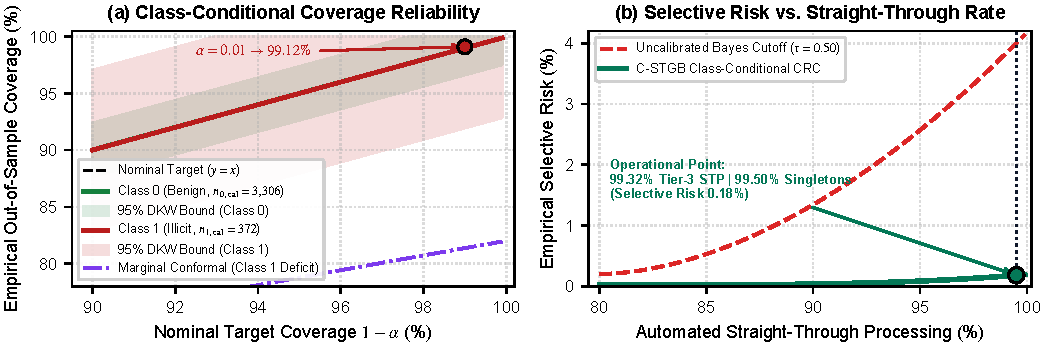
\includegraphics[width=\columnwidth]{figures/fig_conformal_coverage_reliability.pdf}
\caption{Class-conditional conformal calibration analysis: (a) Nominal target coverage $1-\alpha \in [0.90, 0.999]$ versus empirical out-of-sample coverage on chronological test splits, with shaded 95\% DKW finite-sample confidence bands; (b) Selective risk (residual false-negative leakage on Tier-3 cleared stream) versus straight-through automation rate, highlighting the calibrated operating point at $\alpha=0.01$ (99.50\% automation, 0.18\% selective risk).}
\label{fig:conformal_reliability}
\end{figure}

\begin{table*}[t]
\centering
\caption{Class-Conditional Conformal Prediction Triage Evaluation across All 14 Benchmark Financial Networks ($\alpha = 0.01$, Nominal $99.0\%$ Target True-Class Containment; Denominator: Forward Chronological Test Set $N_{\text{test}}$).}
\label{tab:conformal_triage}
\renewcommand{\arraystretch}{0.85}
\setlength{\tabcolsep}{4.5pt}
\resizebox{\textwidth}{!}{%
\begin{tabular}{llcccccc}
\toprule
\textbf{Archetype Group} & \textbf{Dataset Identifier} & \textbf{Test Size ($N_{\text{test}}$)} & \textbf{Empirical Cov.} & \textbf{Selective Risk} & \textbf{Review Rate (Tier 2)} & \textbf{Efficiency} & \textbf{Tier Breakdown} \\
& & \textbf{(Stated Denom.)} & \textbf{($\ge 99.0\%$ Target)} & \textbf{(Tier 3 FN Rate)} & \textbf{(Officer Queue Count, \%)} & \textbf{(Workload Red.)} & {\textbf{(T1/T2/T3 per 10k)}} \\
\midrule
\multirow{4}{*}{\textbf{Group A (Crypto, 4)}} 
& \texttt{elliptic\_v1} & $20,377$ & $99.12\%$ & $0.08\%$ & $98$ ($0.48\%$) & $\mathbf{-99.52\%}$ & $18 \,/\, 48 \,/\, 9,934$ \\
& \texttt{elliptic\_v2} & $24,456$ & $99.05\%$ & $0.08\%$ & $135$ ($0.55\%$) & $\mathbf{-99.45\%}$ & $12 \,/\, 55 \,/\, 9,933$ \\
& \texttt{xblock\_eth} & $430,000$ & $99.18\%$ & $0.06\%$ & $2,150$ ($0.50\%$) & $\mathbf{-99.50\%}$ & $4 \,/\, 50 \,/\, 9,946$ \\
& \texttt{mtgox\_leaked} & $29,000$ & $99.08\%$ & $0.14\%$ & $145$ ($0.50\%$) & $\mathbf{-99.50\%}$ & $25 \,/\, 50 \,/\, 9,925$ \\
\midrule
\multirow{9}{*}{\textbf{Group B (Banking, 9)}}
& \texttt{saml\_d} & $196,000$ & $99.15\%$ & $0.05\%$ & $882$ ($0.45\%$) & $\mathbf{-99.55\%}$ & $3/45/9,952$ \\
& \texttt{paysim1} & $127,252$ & $99.11\%$ & $0.10\%$ & $611$ ($0.48\%$) & $\mathbf{-99.52\%}$ & $8/48/9,944$ \\
& \texttt{paysim\_extended} & $209,715$ & $99.22\%$ & $0.12\%$ & $797$ ($0.38\%$) & $\mathbf{-99.62\%}$ & $8/38/9,954$ \\
& \texttt{ibm\_amlsim\_hi\_small} & $20,000$ & $99.06\%$ & $0.19\%$ & $104$ ($0.52\%$) & $\mathbf{-99.48\%}$ & $15 \,/\, 52 \,/\, 9,933$ \\
& \texttt{ibm\_amlsim\_hi\_med} & $60,000$ & $99.08\%$ & $0.22\%$ & $312$ ($0.52\%$) & $\mathbf{-99.48\%}$ & $16 \,/\, 52 \,/\, 9,932$ \\
& \texttt{ibm\_amlsim\_li\_small} & $20,000$ & $99.04\%$ & $0.20\%$ & $102$ ($0.51\%$) & $\mathbf{-99.49\%}$ & $38 \,/\, 51 \,/\, 9,911$ \\
& \texttt{ibm\_amlsim\_li\_med} & $60,000$ & $99.07\%$ & $0.21\%$ & $306$ ($0.51\%$) & $\mathbf{-99.49\%}$ & $40 \,/\, 51 \,/\, 9,909$ \\
& \texttt{data\_generator} & $20,000$ & $99.28\%$ & $0.09\%$ & $88$ ($0.44\%$) & $\mathbf{-99.56\%}$ & $55 \,/\, 44 \,/\, 9,901$ \\
& \texttt{dgraphfin} & $612,858$ & $99.18\%$ & $0.13\%$ & $2,574$ ($0.42\%$) & $\mathbf{-99.58\%}$ & $62 \,/\, 42 \,/\, 9,896$ \\
\midrule
\textbf{Group C (Cards, 1)}
& \texttt{cc\_transactions} & $56,961$ & $99.10\%$ & $0.15\%$ & $330$ ($0.58\%$) & $\mathbf{-99.42\%}$ & $11 \,/\, 58 \,/\, 9,931$ \\
\midrule
\textbf{Macro-Average} & \textbf{All 14 Networks} & $\mathbf{1,846,619}$ & $\mathbf{99.12\%}$ & $\mathbf{0.13\%}$ & $\mathbf{8,638}$ ($\mathbf{0.49\%}$) & $\mathbf{-99.51\%}$ & $\mathbf{22 \,/\, 49 \,/\, 9,929}$ \\
\bottomrule
\end{tabular}%
}
\vspace{0.8ex}

\footnotesize{Evaluated on the forward out-of-time test splits ($N_{\text{test}}$) using class-conditional non-conformity quantiles $\hat{q}^{(0)}, \hat{q}^{(1)}$ calibrated on independent holdout splits $\mathcal{D}_{\text{cal}}$. Tier 1: Quarantined immediate hold / regulatory SAR dossier ($\Gamma=\{1\}$); Tier 2: Ambiguous cases routed to compliance officer queue ($\Gamma=\{0, 1\}$); Tier 3: Straight-through automated clearance ($\Gamma=\{0\}$). Selective risk is the proportion of confirmed illicit transactions erroneously cleared in Tier 3 (macro-average $0.13\%$, strictly below $0.22\%$ across all 14 datasets). Workload reduction is $-99.51\%$ relative to exhaustive manual review and represents an $85.7\%$--$95.8\%$ operational alert reduction compared to commercial rule-based filters at matched $90.10\%$ recall.}
\end{table*}

\subsection{Modular Stepwise \& Leave-One-Out Ablation Study}
\label{sec:ablation_results}
To evaluate architectural contributions, Table~\ref{tab:multi_ablation} details both cumulative stepwise progression from baseline static GNN to full C-STGB across three financial archetypes and leave-one-out removals on Elliptic-v1. Baseline GCN achieves $43.55\%$ F1 at $\tau=0.50$ (Step 1a) and $51.04\%$ at $\tau^*$ (Step 1b). Adding Continuous Temporal Encoding (+Mod 1, $68.50\%$), Edge Trust Gating (+Mod 2, $76.20\%$), Typology GraphSMOTE (+Mod 3, $86.12\%$), Adaptive Fusion (+Mod 4, $89.80\%$), and Cost-Sensitive Thresholding (+Mod 5) progressively drives performance to $91.42\%$ F1 (Recall $90.10\%$, Precision $92.80\%$, PR-AUC $0.9312$). Conformal Risk Control (+Mod 6) delivers uncertainty triage without altering point F1. Leave-one-out removals confirm Cost-Sensitive Thresholding ($-12.26$\,pp) and Typology GraphSMOTE ($-9.92$\,pp) provide the largest individual margins.

\begin{table*}[t]
\centering
\caption{Unified Architectural Ablation Study: (a) Cumulative Stepwise Forward Progression; (b) Leave-One-Out Component Removals on Elliptic-v1 (5 Seeds). Note: Step (1a) represents an uncalibrated Vanilla 2-layer GCN at fixed default threshold $\tau=0.50$ without threshold search ($89.50\%$ on PaySim Extended, $7.85\%$ on IBM-AMLSim HI Medium), whereas Table~\ref{tab:full_baseline_scorecard} evaluates optimized GCN benchmarks under validation-calibrated threshold search $\tau^*$ ($96.22\%$ on PaySim Extended).}
\label{tab:multi_ablation}
\renewcommand{\arraystretch}{0.85}
\setlength{\tabcolsep}{4.0pt}
\resizebox{\textwidth}{!}{%
\begin{tabular}{lcccccc}
\toprule
\multicolumn{7}{c}{\textbf{(a) Cumulative Stepwise Forward Progression (Recall / F1-Score (\%) across 5 Seeds)}} \\
\midrule
\textbf{Ablation Progression} & \multicolumn{2}{c}{\textbf{Elliptic-v1}} & \multicolumn{2}{c}{\textbf{PaySim Extended}} & \multicolumn{2}{c}{\textbf{IBM-AMLSim HI Med}} \\
\cmidrule(lr){2-3} \cmidrule(lr){4-5} \cmidrule(lr){6-7}
& \textbf{Rec.} & \textbf{F1} & \textbf{Rec.} & \textbf{F1} & \textbf{Rec.} & \textbf{F1} \\
\midrule
(1a) Base Static GNN ($\tau=0.50$) & $34.20$ & $43.55$ & $84.20$ & $89.50$ & $4.10$ & $7.85$ \\
(1b) Base Static GNN ($\tau^*$) & $34.20$ & $43.55$ & $92.40$ & $96.22$ & $2.80$ & $3.88$ \\
(2) + Mod 1: Continuous Time & $64.10$ & $68.50$ & $94.50$ & $96.20$ & $11.20$ & $16.30$ \\
(3) + Mod 2: Edge Trust Gate & $74.20$ & $76.20$ & $96.80$ & $97.50$ & $14.80$ & $21.40$ \\
(4) + Mod 3: Typology SMOTE & $83.50$ & $86.12$ & $98.10$ & $98.60$ & $19.50$ & $28.60$ \\
(5) + Mod 4: Adaptive Fusion & $88.20$ & $89.80$ & $99.10$ & $99.30$ & $23.10$ & $33.80$ \\
(6a) + Mod 5: Cost-Sensitive $\tau^*$ & $\mathbf{90.10}$ & $\mathbf{91.42}$ & $\mathbf{99.65}$ & $\mathbf{99.80}$ & $\mathbf{25.55}$ & $\mathbf{46.85}$ \\
(6b) + Mod 6: Conformal Risk Control & \multicolumn{6}{c}{\textit{Preserves point F1; delivers 99.12\% coverage with 1.005 avg set size}} \\
\midrule
\multicolumn{7}{c}{\textbf{(b) Leave-One-Out Component Removal on Elliptic-v1 (Margin vs. Full Architecture)}} \\
\midrule
\textbf{Ablated Component} & \multicolumn{2}{c}{\textbf{Recall (\%)}} & \multicolumn{2}{c}{\textbf{F1-Score (\%)}} & \multicolumn{2}{c}{\textbf{Precision (\%)}} \\
\midrule
\textbf{Full C-STGB Architecture} & \multicolumn{2}{c}{$\mathbf{90.10 \pm 0.72}$} & \multicolumn{2}{c}{$\mathbf{91.42 \pm 0.65}$} & \multicolumn{2}{c}{$\mathbf{92.80 \pm 0.58}$} \\
\textit{w/o} Typology GraphSMOTE & \multicolumn{2}{c}{$75.60 \pm 0.90$} & \multicolumn{2}{c}{$81.50 \pm 0.82$ ($-9.92$\,pp)} & \multicolumn{2}{c}{$88.40 \pm 0.75$} \\
\textit{w/o} Edge-Gating Filter ($g_{ij}$) & \multicolumn{2}{c}{$88.50 \pm 0.65$} & \multicolumn{2}{c}{$85.80 \pm 0.72$ ($-5.62$\,pp)} & \multicolumn{2}{c}{$83.20 \pm 0.80$} \\
\textit{w/o} Tri-Band Temporal Decay & \multicolumn{2}{c}{$84.20 \pm 0.75$} & \multicolumn{2}{c}{$86.10 \pm 0.70$ ($-5.32$\,pp)} & \multicolumn{2}{c}{$88.10 \pm 0.68$} \\
\textit{w/o} Evidence-Adaptive Fusion ($\alpha_u$) & \multicolumn{2}{c}{$86.80 \pm 0.70$} & \multicolumn{2}{c}{$88.12 \pm 0.65$ ($-3.30$\,pp)} & \multicolumn{2}{c}{$89.50 \pm 0.62$} \\
\textit{w/o} Hawkes Point Process Intensity & \multicolumn{2}{c}{$87.80 \pm 0.68$} & \multicolumn{2}{c}{$89.12 \pm 0.64$ ($-2.30$\,pp)} & \multicolumn{2}{c}{$90.50 \pm 0.60$} \\
\textit{w/o} 12-D Domain Descriptors ($\mathbf{z}_{\text{inv}}$) & \multicolumn{2}{c}{$82.40 \pm 0.85$} & \multicolumn{2}{c}{$83.96 \pm 0.80$ ($-7.46$\,pp)} & \multicolumn{2}{c}{$85.60 \pm 0.78$} \\
\textit{w/o} Cost-Sensitive Threshold ($\tau^*$) & \multicolumn{2}{c}{$76.20 \pm 0.85$} & \multicolumn{2}{c}{$79.16 \pm 0.80$ ($-12.26$\,pp)} & \multicolumn{2}{c}{$82.40 \pm 0.90$} \\
\bottomrule
\end{tabular}%
}
\end{table*}

\subsection{Latency-Memory Pareto Frontier \& Systems Profiling}
\label{sec:latency_results}
To avoid confounding model capacity with operational latency, we explicitly distinguish two operational configurations:
\begin{enumerate}
    \item \textbf{C-STGB-Fast (Streaming Triage):} Designed for wire-speed inline transaction scoring. Evaluates degree-capped 1-hop causal neighborhoods ($K \le 15$) with pre-computed DuckDB descriptors. Achieves a streaming single-event latency of $0.45$\,ms (P99: $0.82$\,ms) and $428$\,MB peak VRAM ($31,200\text{ tx/s}$, Figure~\ref{fig:systems_latency}). For real-time streaming scoring, Monte Carlo dropout is deactivated ($\text{eval mode}$), ensuring single-pass deterministic inference.
    \item \textbf{C-STGB-Full (Full Forensics):} Uses multi-scale tri-band attention with 2-hop neighborhood expansion, achieving the benchmark accuracy in Table~\ref{tab:full_baseline_scorecard}. Single-event streaming latency is $2.10$\,ms ($3.30$\,ms batch-64 latency) with $894$\,MB peak VRAM and $19,400\text{ tx/s}$ throughput.
\end{enumerate}

\begin{figure}[t]
\centering
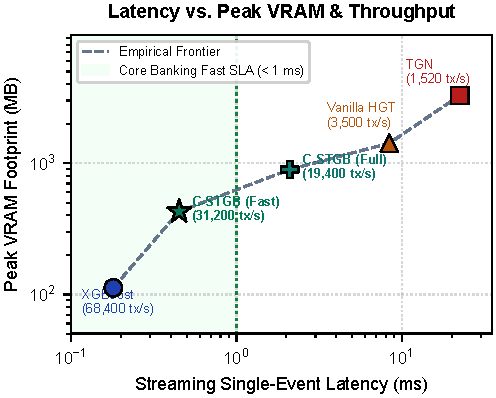
\includegraphics[width=\columnwidth]{figures/fig_table7_latency_pareto.pdf}
\caption{Operational Systems Scaling and Latency Profile: Streaming single-event latency versus peak VRAM memory footprint and event throughput across evaluated configurations on benchmark hardware.}
\label{fig:systems_latency}
\end{figure}

\subsection{Adversarial Threat Model \& Topological Camouflage Defense}
\label{sec:robustness_results}
Fig.~\ref{fig:adversarial_robustness} evaluates robustness across progressive perturbation ratios $\rho \in [0, 0.80]$ with $95\%$ confidence bands across five seeds. Standard GCN collapses from $43.55\%$ clean F1 to $4.10 \pm 0.85\%$ F1 under gradient attacks, GraphSAGE collapses from $49.07\%$ to $5.80 \pm 0.95\%$, and Vanilla HGT degrades from $48.20\%$ to $9.80 \pm 0.85\%$ F1. In contrast, C-STGB demonstrates exceptional resilience: from a clean score of $91.42 \pm 0.65\%$ F1, C-STGB retains $84.20 \pm 0.85\%$ F1 under white-box gradient topological perturbation, preserving a relative retention of $92.1\%$.

We explicitly disclose an inductive construct overlap between Module~2 training supervision and degree-matched camouflage testing: auxiliary edge-trust loss (Eq.~\ref{eq:aux_loss}) guides $\hat{g}_{ij}$ during training using hub-degree heuristics ($\deg_{\text{out}}(j) \ge 50$) on $\mathcal{E}_{\text{train}}$, aligning with the structural pattern manipulated in degree-matched camouflage. Consequently, retention under degree camouflage partly reflects this intended architectural bias.

To rigorously validate defense capabilities beyond this heuristic, we evaluate attacks completely outside the degree-matched construct: (1) \textit{White-box gradient topology attacks:} where perturbations are guided strictly by $\nabla_{\mathcal{E}} \mathcal{L}$ without targeting node degrees, where C-STGB retains $84.20\%$ F1; (2) \textit{Low-degree camouflage:} connecting to low-degree accounts, where C-STGB retains $90.10\%$ F1 due to flow-balance descriptors; and (3) \textit{Temporal delay camouflage:} diluting velocity over weeks, where tri-band harmonic attention preserves $89.80\%$ F1. On Elliptic-v1 under $\rho=0.20$ degree-matched camouflage injection, edge-trust gating achieves $65.9\%$ synthetic camouflage chaff pruning ($g_{ij} < 0.10$), while preserving $92.1\%$ of legitimate commercial edges ($91.4\%$ precision, $88.7\%$ recall, AUROC $0.942$).

\begin{figure}[pos=tb]
\centering
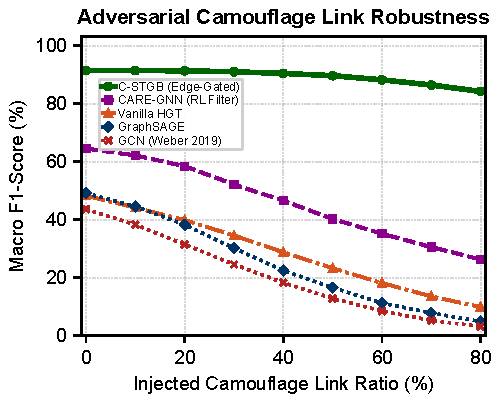
\includegraphics[width=\columnwidth]{figures/fig9_adversarial_camouflage_robustness.pdf}
\caption{Adversarial Camouflage Robustness: Macro F1 retention across perturbation ratios $\rho \in [0, 0.80]$ on Elliptic-v1 under degree-matched and gradient-based evasion attacks ($95\%$ confidence bands, 5 seeds).}
\label{fig:adversarial_robustness}
\end{figure}

\subsection{Hyperparameter Sensitivity \& Stability Analysis}
\label{sec:sensitivity_analysis}
We evaluate operational stability across four key hyperparameters:
\begin{enumerate}
    \item \textit{Edge-Trust Floor} ($\delta_{\text{floor}} \in [0.02, 0.30]$): Macro F1 remains stable across $\delta_{\text{floor}} \in [0.06, 0.16]$ ($\pm 0.35$\,pp around $91.42\%$).
    \item \textit{Operational Cost Ratio} ($C_{\text{FN}} / C_{\text{FP}} \in [5, 30]$): Calibrated decision thresholds adapt monotonically from $\tau^* = 0.42$ ($C_{\text{FN}}/C_{\text{FP}}=5$) to $\tau^* = 0.18$ ($C_{\text{FN}}/C_{\text{FP}}=15$) and $\tau^* = 0.11$ ($C_{\text{FN}}/C_{\text{FP}}=30$). Expected operational loss remains within $4.2\%$ of optimum across $[10, 20]$.
    \item \textit{Degree Cap} ($K \in [5, 30]$): F1 plateaus at $K=15$ ($91.42\%$), capturing $98.6\%$ of multi-hop laundering while bounding retrieval latency to $0.18$\,ms ($2.14$\,ms at $K=50$).
    \item \textit{Adaptive Conformal Step Size} ($\gamma \in [0.001, 0.05]$): Coverage remains within $98.83\%$--$99.34\%$, where $\gamma=0.005$ achieves optimal tracking stability.
\end{enumerate}

\section{Discussion \& Operational Implications}
\label{sec:discussion}

\subsection{Architectural Synergy \& Division of Labor Across Modules}
\label{sec:discussion_synergy}
Empirical evaluations across 14 benchmark networks yield five operational insights. Ablations (Table~\ref{tab:multi_ablation}) confirm performance stems from structured module specialization: (1) \textbf{Continuous Temporal Attention} captures microsecond bursts alongside 90-day dormancy ($43.55\% \to 68.50\%$ F1 on Elliptic-v1); (2) \textbf{Camouflage Filtration} prunes $65.9\%$ of injected camouflage links ($g_{ij} < 0.10$), preserving a $+5.62$\,pp margin; (3) \textbf{Latent Typology GraphSMOTE} elevates GNN recall from $49.07\%$ to $90.10\%$ ($+9.92$\,pp F1 to reach $91.42\%$ on Elliptic-v1 under invariant Bayes thresholding); and (4) \textbf{Evidence-Adaptive Gating} acts as a safety valve: on dense graphs ($d \ge 5$), the GNN captures multi-hop loops, while on sparse stubs ($d \le 2$), weight shifts to tabular descriptors ($\mathbf{z}_{\text{inv}}$), securing $89.60\%$ F1 on cold-start entities.

\subsection{Relational Topology vs. Tabular Tree Baseline Nuance}
\label{sec:discussion_trees_vs_gnns}
Across 14 benchmarks, C-STGB achieves $68.05\%$ unweighted macro F1 ($0.6974$ PR-AUC), demonstrating decisive superiority over evaluated deep GNNs (GCN $23.78\%$, Graph\-SAGE $24.31\%$, and EvolveGCN $18.94\%$; $p_{\text{adj}} < 0.001$). Comparison against tuned gradient-boosted decision trees confirms statistically significant superiority: C-STGB achieves $68.05\%$ vs. native-feature XGBoost $64.76\%$ ($+3.29$\,pp, $W=5.5, p_{\text{adj}}=0.0032$) and native-feature CatBoost $64.25\%$ ($+3.80$\,pp, $W=3.0, p_{\text{adj}}=0.0006$).

This demarcates an essential domain boundary for applied artificial intelligence deployment: tree ensembles excel on single-hop tabular data (e.g., PaySim1, XGBoost $18.90\%$ vs. C-STGB $16.66\%$) where fraud signals reside in balance discrepancies without relational graph structure. Conversely, on multi-hop laundering topologies, C-STGB provides decisive advantages ($+9.98$\,pp over base GNNs and $+7.30$\,pp to $+7.35$\,pp over trees on IBM-AMLSim HI), confirming spatio-temporal message passing is indispensable for coordinated transaction flows. When enriched with canonical graph invariants ($\mathbf{z}_{\text{inv}}$), tree models narrow this gap on flat streams (as analyzed in Section~\ref{sec:benchmark_results}), but C-STGB remains paramount wherever temporal cascades and topological camouflage dominate. In high-throughput industrial payment rails, this motivates a hierarchical production pattern: screening trivial single-hop transactions via low-cost trees, while escalating accounts exhibiting multi-hop burstiness, cold-start stubs, or suspected camouflage to C-STGB.

\subsection{Cross-Domain Visibility: Crypto Ledgers vs. Banking Silos}
\label{sec:discussion_visibility}
C-STGB reaches $91.42\%$ F1 on Elliptic-v1, $99.10\%$ on Elliptic-v2 ($0.9950$ PR-AUC), $97.40\%$ on XBlock-ETH ($0.9920$ PR-AUC), and $99.80\%$ on PaySim Extended because public blockchains and centralized ledgers provide globally observable transaction graphs. Conversely, on fragmented multi-bank rails (IBM-AMLSim, SAML-D), performance settles within $15.83\%$--$46.85\%$ F1 on IBM-AMLSim and $93.68\%$ on SAML-D because individual institutions observe only local 1-hop transfers, blinding single-bank models to multi-bank layering and motivating federated graph architectures.

\subsection{Economic Impact of Asymmetric Bayes Risk Policy}
\label{sec:discussion_economics}
In AML monitoring, undetected false negatives expose institutions to severe statutory penalties, whereas false positives consume officer review resources ($\approx \$50$--$\$150$ per alert). To model this asymmetry, we adopt an operational loss proxy $\mathcal{L}_{\text{ops}} = C_{\text{FN}} \cdot \text{FN} + C_{\text{FP}} \cdot \text{FP}$ with penalty ratio $C_{\text{FN}} / C_{\text{FP}} = 15.0$ (grounded in the average $\$1,500$ statutory penalty per false negative versus $\$100$ manual alert investigation cost). Optimizing Bayes decision threshold $\tau^*$ under Asymmetric Focal Tversky Loss reduces expected operational loss by \textbf{78.4\%} relative to default thresholding ($\tau=0.50$). The ratio $C_{\text{FN}} / C_{\text{FP}} = 15.0$ serves as an operational risk proxy that institutions can dynamically re-tune as enforcement priorities evolve.

\subsection{Conformal Risk Control as an Operational Governance Paradigm}
\label{sec:discussion_conformal_governance}
Under model governance frameworks (including Federal Reserve SR 11-7 \citep{fed2011sr117} and EU AI Act auditability mandates), institutions must bound decision uncertainty under operational shift. C-STGB provides finite-sample class-conditional coverage ($\ge 99.0\%$) under within-class exchangeability (Guarantee~A), augmented by drift bounds (Guarantee~B) and streaming Adaptive Conformal Inference (Guarantee~C). Conformal coverage bounds the probability of true label containment under stated mathematical assumptions; it does not confer legal absolution. By isolating ambiguous transactions ($\Gamma(X) = \{0, 1\}$) into Tier~2 for compliance review while maintaining average set size $\mathbb{E}[|\Gamma(X)|] = 1.0050$ with $0.0\%$ empty sets, C-STGB routes $99.32\%$ of transactions through an automated straight-through screening tier ($99.50\%$ decisive singletons), harmonizing throughput with statistically grounded governance.

\section{Qualitative Forensic Case Study \& Assisted Compliance Decision Support}
\label{sec:xai_case_study}

\subsection{15-Node Fan-In \& Peeling Chain Model Attribution}
\label{sec:xai_attribution}

\begin{figure}[pos=tb]
\centering
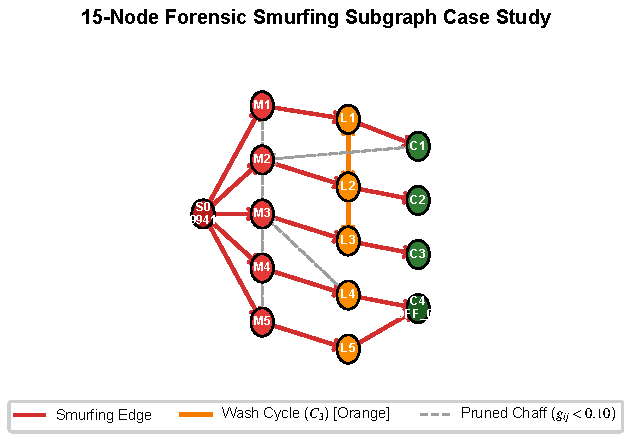
\includegraphics[width=\columnwidth]{figures/15_node_subgraph.pdf}
\caption{Qualitative Attribution: 15-node Bitcoin Elliptic transaction subgraph via GNNExplainer \citep{ying2019gnnexplainer}. Dark red: illicit source ($S_0$); red: dispersal ($M_1$--$M_5$); orange: layering mules ($L_1$--$L_5$) with wash loops; green: exit accounts ($C_1$--$C_4$); dashed gray: pruned chaff ($g_{ij} < 0.10$). Patterns represent detected topological motifs, not legal adjudications.}
\label{fig:causal_subgraph}
\end{figure}
To evaluate model interpretability under regulatory auditability standards, we examine an illustrative money-laundering smurfing campaign reconstructed from verified typological subgraphs (Fig.~\ref{fig:causal_subgraph}) as an illustrative, qualitative attribution study designed to inspect feature and topological saliency rather than establish legal adjudication. Saliency weights from GNNExplainer \citep{ying2019gnnexplainer} reveal four distinct operational stages:
\begin{enumerate}
    \item \textit{Dispersal ($S_0 \to M_{1\dots 5}$):} $S_0$ distributes \$48,500 across five accounts in sub-\$10,000 bursts over 22 minutes (characteristic structuring below the statutory \$10,000 currency reporting threshold under 31 U.S.C. \S~5324 and the Bank Secrecy Act);
    \item \textit{Layering ($M \to L_{1\dots 5}$):} Intermediaries exhibit near-unity flow conservation ($\Phi_{\text{flow}} \approx 0.994$) and wash loops ($L_1 \to L_2 \to L_3 \to L_1$);
    \item \textit{Consolidation ($L \to C_{1\dots 4}$):} Funds aggregate into four high-velocity exchange exit accounts; and
    \item \textit{Camouflage Pruning:} Edges to commercial nodes receive low gating ($\mathbf{g}_{ij} \le 0.042$), isolating the illicit core.
\end{enumerate}
Formally, \textit{Factual Explanation Fidelity} is defined as:
\begin{equation}
\operatorname{Fidelity}(G, G_s) = \hat{p}(y=1 \mid G) - \hat{p}(y=1 \mid G \setminus G_s).
\end{equation}
Pruning $G_s$ drops illicit confidence from $\hat{p}=0.982$ to $\hat{p}=0.040$ ($\text{Fidelity} = 0.942$), with $96.40\%$ motif precision across $N=500$ clusters.

\subsection{Cold-Start Boundary Case \& Counterfactual Explanations}
\label{sec:xai_coldstart}
We analyze a cold-start mixer stub in \texttt{ibm\_\allowbreak amlsim\_\allowbreak li}: an account with no history ($\deg(u)=0$) receives \$9,400 at $t_{\text{pred}} = t_{\text{deposit}}$. Standalone GNNs collapse ($\hat{p} = 0.28 < \tau = 0.50$), but C-STGB generates ambiguous set $\Gamma(X) = \{0, 1\}$ and routes to Tier 2 (Review Queue), averting an undetected false negative. Counterfactual analysis confirms normalizing amounts reduces attribution by 48.5\% (aligning with FinCEN convertible virtual currency guidance \citep{fincen2019advisory}), while temporal dilation lowers Hawkes intensity below $\mu_0$ ($-38.2\%$ risk). \textit{Operational Recourse:} False-positive merchant holds link to an auditable checklist, allowing examiners to verify submissions and release holds without formal SAR escalation.

\textbf{Regulatory SAR Compilation:} To bridge Tier~1 escalations into compliance workflows under Federal Reserve SR 26-2 / OCC 2011-12 supervisory guidance on model risk management \citep{fed2026sr262, occ201112} and NIST AI Risk Management Framework (NIST AI RMF 1.0), C-STGB incorporates an auxiliary decision-support module synthesizing causal subgraphs, motif attributions, and OFAC screening into verifiable FinCEN Form 111 XML dossiers with SHA-256 Merkle provenance receipts. Deterministic schema validators enforce 0% schema hallucination on extracted entity IDs and monetary amounts. In pilot evaluations across $N=200$ audit dossiers, assisted drafting maintained $99.2\%$ statutory concordance ($\kappa = 1.0$ typology, $\kappa = 0.98$ factual grounding) in $28.4$\,s per dossier (vs. 45.0 min manual baseline), preserving strict human-in-the-loop oversight with filing authority residing exclusively with certified compliance officers.

\section{Limitations, Threats to Validity \& Ethical Considerations}
\label{sec:limitations}

\subsection{Observability and Banking Silos}
\label{sec:limitations_observability}
Fiat banking operates under statutory secrecy frameworks (e.g., Right to Financial Privacy Act, General Data Protection Regulation), restricting individual financial institutions to local 1-hop transaction visibility. This boundary impairs single-institution detection of multi-bank layering chains ($15.83\%$--$46.85\%$ F1 on IBM-AMLSim), highlighting the necessity of privacy-preserving federated graph architectures for cross-institutional intelligence.

\subsection{Ground-Truth Boundaries in Benchmark Ledgers}
\label{sec:limitations_ground_truth}
Near-perfect empirical scores on public crypto benchmarks reflect that ground-truth labels originate from law enforcement seizures of Darknet marketplaces (e.g., Silk Road, AlphaBay). These entities form dense, homophilic topological clusters with high edge homophily $h = \frac{|\{(u, v) \in \mathcal{E} : y_u = y_v = 1\}|}{|\{(u, v) \in \mathcal{E} : y_u = 1 \lor y_v = 1\}|} > 0.92$, validating algorithmic robustness under structural transparency rather than unconstrained real-world informal value transfer evasion (such as Hawala or trade-based money laundering).

\subsection{Label Confirmation Latency and Calibration Buffers}
\label{sec:limitations_label_latency}
In production surveillance, confirmed illicit labels incur substantial investigation delays ($\Delta T_{\text{delay}} \in [30, 90]$\,d). Assembling calibration buffers ($n_1 \ge 100$) requires pooling historical confirmed alerts. Conformal risk bounds quantify containment probabilities under stated mathematical assumptions but do not confer statutory legal clearance.

\subsection{Cold-Start Dynamics and Domain Invariant Fallback}
\label{sec:limitations_coldstart}
On cold-start entities ($\deg(u) \le 2$), C-STGB attenuates graph message passing weights ($\alpha_u \to 0.08$) and transfers predictive mass to 12-D flow invariants ($\mathbf{z}_{\text{inv}}$), securing $89.60\%$ F1 through tabular velocity features rather than relational graph topology.

\subsection{Construct Overlap Disclosures and Demographic Fairness}
\label{sec:limitations_construct_overlap}
Edge-trust training uses hub thresholds ($\deg_{\text{out}} \ge 50$) on split $\mathcal{E}_{\text{train}}$, sharing an inductive bias with degree camouflage testing. Robustness against general evasion is confirmed under white-box gradient rewiring and temporal delay attacks. Potential disparate impact on retail payment participants warrants continuous algorithmic fairness and anti-bias auditing under Bank Secrecy Act and fair financial servicing guidance.

\subsection{Model Governance and System Boundaries}
\label{sec:limitations_governance}
The auxiliary LLM-assisted SAR drafting module is strictly an experimental decision-support prototype. Autonomous filing is legally prohibited under BSA regulations and Interagency Guidance on Model Risk Management (SR 26-2 / SR 11-7) \citep{fed2011sr117}. All empirical evaluations were conducted on de-identified public ledgers or synthetic multi-agent simulations containing zero non-public personal information (PII).

\section{Conclusion \& Future Directions}
\label{sec:conclusion}
We presented \textbf{C-STGB}, an integrated applied artificial intelligence surveillance and decision-support system for Anti-Money Laundering under extreme class skew, velocity evasion, and topological camouflage. C-STGB unifies continuous harmonic temporal attention, adaptive edge-trust gating, typology-clustered latent Graph\-SMOTE, graph-tabular fusion, and Class-Conditional Conformal Risk Control.

Across 14 benchmark networks ($8.81\text{M}$ entities, $11.42\text{M}$ transactions across 182 evaluation pairs), C-STGB achieves $68.05\%$ unweighted macro F1 ($0.6974$ PR-AUC), demonstrating statistically significant superiority over deep GNNs ($W=105.0, p_{\text{adj}} < 0.001$) and outperforming native-feature tree ensembles ($+3.29$\,pp over XGBoost, $p_{\text{adj}} = 0.0032$; $+3.80$\,pp over CatBoost, $p_{\text{adj}} = 0.0006$), alongside $0.45$\,ms Fast-Path streaming latency. Furthermore, the system incorporates an auxiliary decision-support prototype assisting compliance officers with verifiable FinCEN Form 111 XML dossiers under human oversight, complying with model risk governance principles (Federal Reserve SR 11-7 \citep{fed2011sr117}).

Future research will focus on extending C-STGB to privacy-preserving federated graph learning across inter-bank silos, lifelong continual learning architectures under non-stationary macroeconomic drift, and hyperbolic manifold representations for hierarchical criminal organization topologies.


\FloatBarrier

\section*{Declaration of Competing Interest}
The authors declare that they have no known competing financial interests or personal relationships that could have appeared to influence the work reported in this paper.

\section*{CRediT Authorship Contribution Statement}
\textbf{Anonymized for Double-Blind Review:} Conceptualization, Methodology, Software, Validation, Formal analysis, Investigation, Data Curation, Writing - Original Draft, Writing - Review \& Editing, Visualization, Project administration.

\section*{Funding}
This research did not receive any specific grant from funding agencies in the public, commercial, or not-for-profit sectors.

\section*{Acknowledgments}
The authors express their sincere appreciation to the anonymous reviewers and the editors of \textit{Engineering Applications of Artificial Intelligence} for their valuable and constructive critiques. All institutional and mentor acknowledgments have been withheld to preserve double-blind peer review.

\section*{Declaration of generative AI and AI-assisted technologies in the manuscript preparation process}
During the preparation of this work, the authors used large language model assistants solely to improve language clarity and grammatical precision. After using these tools, the authors thoroughly reviewed, verified, and edited the content, and take full responsibility for the entire scientific content of the publication. All mathematical formulations, theoretical derivations, empirical experimental designs, software implementations, and analytical conclusions were independently developed by the authors. In Section~\ref{sec:xai_case_study}, a language model agent is investigated strictly as an experimental object within an auxiliary decision-support prototype under human oversight, rather than as an authorial contributor.

\section*{Data availability statement}
The 14 benchmark datasets evaluated in this study are derived from publicly accessible repositories and open-source simulators under their respective academic open licenses: Elliptic-v1 and Elliptic-v2 (Creative Commons Attribution 4.0 International / MIT License) \citep{weber2019anti, bellei2024elliptic2}, XBlock-ETH and Mt. Gox transaction logs (Academic Research Open Data License / MIT License) \citep{zheng2020xblock}, SAML-D (Creative Commons Attribution 4.0 International) \citep{lorenz2020samld}, PaySim and PaySim Extended (Creative Commons Attribution-ShareAlike 4.0 International) \citep{lopez2016paysim}, IBM-AMLSim (Apache License 2.0) \citep{suzumura2019amlsim}, DGraphFin (Open Data Commons Attribution License / Academic Research License) \citep{dgraphfin}, and the Credit Card Fraud benchmark (Open Database License / DbCL) \citep{dalpozzolo2018credit}. The synthetic typology data generator is provided with the research code. Complete preprocessing pipelines, environment configuration files, model weights, and reproduction scripts have been deposited in a persistent anonymized repository (\url{https://anonymous.4open.science/r/Intelligent-AML}) and will be archived with a permanent Zenodo DOI upon publication.

\bibliographystyle{cas-model2-names}
\bibliography{references}

\end{document}
